%% Customizacoes do abnTeX2 (http://abnTeX2.googlecode.com) para o IFRS Campus Osorio v1.1
%% Por Bruno Fernandes (bruno.fernandes@osorio.ifrs.edu.br)
%% O modelo mais atualizado está disponível em bit.ly/ADSLaTeX
%%
%% abtex2-modelo-trabalho-academico.tex, v-1.9.6 laurocesar
%% Copyright 2012-2016 by abnTeX2 group at http://www.abntex.net.br/ 
%%
%% This work may be distributed and/or modified under the
%% conditions of the LaTeX Project Public License, either version 1.3
%% of this license or (at your option) any later version.
%% The latest version of this license is in
%%   http://www.latex-project.org/lppl.txt
%% and version 1.3 or later is part of all distributions of LaTeX
%% version 2005/12/01 or later.
%%
%% This work has the LPPL maintenance status `maintained'.
%% 
%% The Current Maintainer of this work is the abnTeX2 team, led
%% by Lauro César Araujo. Further information are available on 
%% http://www.abntex.net.br/
%%
%% This work consists of the files abntex2-modelo-trabalho-academico.tex,
%% abntex2-modelo-include-comandos and abntex2-modelo-references.bib
%%

% ------------------------------------------------------------------------
% ------------------------------------------------------------------------
% abnTeX2: Modelo de Trabalho Academico (tese de doutorado, dissertacao de
% mestrado e trabalhos monos em geral) em conformidade com 
% ABNT NBR 14724:2011: Informacao e documentacao - Trabalhos academicos -
% Apresentacao
% ------------------------------------------------------------------------
% ------------------------------------------------------------------------

\documentclass[
	% -- opções da classe memoir --
	12pt,				% tamanho da fonte
	openright,			% capítulos começam em pág ímpar (insere página vazia caso preciso)
	% twoside,			% para impressão em recto e verso. Oposto a oneside. FRENTE E VERSO
    oneside,			% para impressão em apenas um lado. APENAS FRENTE
	a4paper,			% tamanho do papel. 
	% -- opções da classe abntex2 --
	chapter=TITLE,		% títulos de capítulos convertidos em letras maiúsculas
	section=TITLE,		% títulos de seções convertidos em letras maiúsculas
	% -- opções do pacote babel --
	english,			% idioma adicional para hifenização
	french,				% idioma adicional para hifenização
	spanish,			% idioma adicional para hifenização
	brazil				% o último idioma é o principal do documento
	]{abntex2}


\usepackage{customizacoes-ifrs-osorio}
\usepackage[expansion=false]{microtype}
\usepackage{float}
% ---
% Pacotes básicos 
% ---
\usepackage{longtable}
\usepackage{wasysym}
\usepackage[table]{xcolor}
\usepackage{tgtermes}		
\usepackage[T1]{fontenc}		% Selecao de codigos de fonte.
\usepackage[utf8]{inputenc}		% Codificacao do documento (conversão automática dos acentos)
\usepackage{lastpage}			% Usado pela Ficha catalográfica
\usepackage{indentfirst}		% Indenta o primeiro parágrafo de cada seção.
\usepackage{color}				% Controle das cores
\usepackage{graphicx}			% Inclusão de gráficos
\usepackage{microtype} 			% para melhorias de justificação
\renewcommand{\ABNTEXchapterfont}{\fontfamily{ptm}\fontseries{sbc}\selectfont}
% ---

% ----------------------------------------------
% Configuração das fontes
% ----------------------------------------------
% Algumas configurações de fontes para capitulos e seções
\renewcommand{\ABNTEXchapterfontsize}{\normalsize\bfseries}
\renewcommand{\ABNTEXpartfontsize}{\ABNTEXchapterfontsize}
\renewcommand{\ABNTEXsectionfontsize}{\normalsize}
\renewcommand{\ABNTEXsubsectionfontsize}{\normalsize\bfseries}
\renewcommand{\ABNTEXsubsubsectionfont}{\slshape\bfseries}
\renewcommand{\ABNTEXsubsubsubsectionfont}{\slshape}

% ---
% Pacotes adicionais, usados apenas no âmbito do Modelo Canônico do abnteX2
% ---
\usepackage{lipsum}				% para geração de dummy text
% ---

%pacote para inserir blocos de código
\usepackage{listings}
\usepackage{color}

\usepackage{textcomp}

\usepackage[font=small]{caption}

% ---
% Pacotes de citações
% ---
\usepackage[brazilian,hyperpageref]{backref}	 % Paginas com as citações na bibl
\usepackage[alf]{abntex2cite}	% Citações padrão ABNT


% --- 
% CONFIGURAÇÕES DE PACOTES
% --- 

%Configurações do pacote listings
%New colors defined below
\definecolor{codegreen}{rgb}{0,0.6,0}
\definecolor{codegray}{rgb}{0.5,0.5,0.5}
\definecolor{codered}{rgb}{0.8,0.1,0.3}
\definecolor{backcolour}{rgb}{0.96,0.96,0.93}

%Code listing style named "mystyle"
\lstdefinestyle{mystyle}{
	backgroundcolor=\color{backcolour},   
	commentstyle=\color{codegreen},
	keywordstyle=\bfseries\color{blue},
	numberstyle=\tiny\color{codegray},
	stringstyle=\color{codered},
	basicstyle=\footnotesize\ttfamily,
	breakatwhitespace=false,         
	breaklines=true,                 
	captionpos=t, 
	keepspaces=true,                 
	numbers=left,                    
	numbersep=5pt,
	showspaces=false,                
	showstringspaces=false,
	showtabs=false,                  
	tabsize=2,
	numberbychapter=false
}
\lstset{style=mystyle}
\renewcommand{\lstlistingname}{Código}

% ---
% Configurações do pacote backref
% Usado sem a opção hyperpageref de backref
\renewcommand{\backrefpagesname}{Citado na(s) página(s):~}
% Texto padrão antes do número das páginas
\renewcommand{\backref}{}
% Define os textos da citação
\renewcommand*{\backrefalt}[4]{
	\ifcase #1 %
		Nenhuma citação no texto.%
	\or
		Citado na página #2.%
	\else
		Citado #1 vezes nas páginas #2.%
	\fi}%
% ---

% ---
% Informações de dados para CAPA e FOLHA DE ROSTO
% ---
\titulo{AutoForm- Sistema para o Registro de Produtos Controlados no SIGMA via Arquivo Eletrônico em Lote (AEL) da Brigada Militar do RS }
\autor{Erik Barcella}
\local{Osório}
\data{2023}
\orientador{Bruno Chagas Fernandes}
\coorientador{Márcio José de Lemos}

\instituicao{%
  Instituto Federal de Educação, Ciência e Tecnologia do Rio Grande do Sul -- IFRS
  \par
  \textit{Campus} Osório
  \par
  Curso Superior de Tecnologia em Análise e Desenvolvimento de Sistemas}
\tipotrabalho{Trabalho de Conclusão de Curso}
% O preambulo deve conter o tipo do trabalho, o objetivo, 
% o nome da instituição e a área de concentração 
\preambulo{Trabalho de Conclusão de Curso apresentado como requisito parcial para obtenção do título de Tecnólogo em Análise e Desenvolvimento de Sistemas.}
% ---


% ---
% Configurações de aparência do PDF final

% alterando o aspecto da cor azul
\definecolor{blue}{RGB}{41,5,195}

% informações do PDF
\makeatletter
\hypersetup{
     	%pagebackref=true,
		pdftitle={\@title}, 
		pdfauthor={\@author},
    	pdfsubject={\imprimirpreambulo},
	    pdfcreator={LaTeX with abnTeX2},
		pdfkeywords={trabalho de concusão de curso}{ifrs}{campus osório}{ads}{análise e desenvolvimento de sistemas}, %adicionar as keywords do trabalho
		colorlinks=true,       		% false: boxed links; true: colored links
    	linkcolor=blue,          	% color of internal links
    	citecolor=blue,        		% color of links to bibliography
    	filecolor=magenta,      		% color of file links
		urlcolor=blue,
		bookmarksdepth=4
}
\makeatother
% --- 

% --- 
% Espaçamentos entre linhas e parágrafos 
% --- 
% O tamanho do parágrafo é dado por:
\setlength{\parindent}{1.3cm}
% Controle do espaçamento entre um parágrafo e outro:
\setlength{\parskip}{0.2cm}  % tente também \onelineskip

% ---
% compila o indice
% ---
\makeindex
% ---

% ----
% Início do documento
% ----
\begin{document}

% Seleciona o idioma do documento (conforme pacotes do babel)
%\selectlanguage{english}
\selectlanguage{brazil}

% Retira espaço extra obsoleto entre as frases.
\frenchspacing 

% ----------------------------------------------------------
% ELEMENTOS PRÉ-TEXTUAIS
% ----------------------------------------------------------
% \pretextual

% ---
% Capa ((Obrigatório)
% ---
\imprimircapa
% ---

% ---
% Folha de rosto (Obrigatório)
% (o * indica que haverá a ficha bibliográfica)
% ---
\imprimirfolhaderosto*

% Inserir errata (Opcional)
% ---
%\input{elementos-pre-textuais/errata}
% ---

% ---
% Inserir folha de aprovação (Obrigatório)
% ---
% Isto é um exemplo de Folha de aprovação, elemento obrigatório da NBR
% 14724/2011 (seção 4.2.1.3).
%
\begin{folhadeaprovacao}

  \begin{center}
    {\ABNTEXchapterfont\large\imprimirautor}

    \vspace*{\fill}\vspace*{\fill}
    \begin{center}
      \ABNTEXchapterfont\bfseries\Large\imprimirtitulo
    \end{center}
    \vspace*{\fill}
    
    \hspace{.45\textwidth}
    \begin{minipage}{.5\textwidth}
        \imprimirpreambulo
    \end{minipage}%
    \vspace*{\fill}
   \end{center}
     
   %Adicionar o texto abaixo depois do trabalho ser aprovado pela banca.   
   %Trabalho aprovado. \imprimirlocal, xx de xxxxxxxxx de 201X:

   \assinatura{\textbf{\imprimirorientador} \\ Orientador} 
   \assinatura{\textbf{\imprimircoorientador} \\ Coorientador } 
   \assinatura{\textbf{Tiago Guimarães Moraes} \\ Convidado 1}
   \assinatura{\textbf{Marcelo Paravisi} \\ Convidado 2}
   %\assinatura{\textbf{Professor} \\ Convidado 3}
   %\assinatura{\textbf{Professor} \\ Convidado 4}
    
    \vspace*{1.5cm}
   \begin{center}
    \vspace*{0.5cm}
    {\large\imprimirlocal}
    \par
    {\large\imprimirdata}
    \vspace*{1cm}
  \end{center}
  
\end{folhadeaprovacao}
% ---

% ---
% Dedicatória (Opcional)
% ---
\begin{dedicatoria}
   \vspace*{\fill}
   \centering
   \noindent
   \textit{ Este trabalho é dedicado a...} \vspace*{\fill}
\end{dedicatoria}
% ---

% ---
% Agradecimentos (Opcional)
% ---
\begin{agradecimentos}
    Os agradecimentos principais são destinados à minha esposa Vitória e à minha família, que estiveram sempre ao meu lado, proporcionando apoio e incentivo ao longo desta jornada. Vocês são a minha base, as fontes constantes de inspiração que tornaram possível alcançar este objetivo
    
    Agradeço imensamente ao Sd. Tiago Costa dos Santos por ser o elo de idealização deste trabalho junto à Brigada Militar, fornecendo apoio e suporte essenciais para a conclusão deste projeto. Sua colaboração foi fundamental para a realização deste trabalho.

    Aos meus dedicados orientador e coorientador, Bruno Chagas Alves Fernandes e Márcio José de Lemos, expresso profundos agradecimentos. Suas orientações foram cruciais, e a dedicação, paciência e contribuições de ambos enriqueceram significativamente este trabalho. Agradeço pelo comprometimento e pelos valiosos ensinamentos que foram essenciais para o sucesso deste projeto acadêmico.

    Agradeço também a todos os demais que contribuíram de alguma forma para que isso fosse possível.




\end{agradecimentos}
% ---

% ---
% Epígrafe (Opcional)
% ---
\begin{epigrafe}
    \vspace*{\fill}
    \begin{flushright}
        \textit{''Só se pode alcançar um grande êxito quando nos mantemos fiéis a nós mesmos'' - Friedrich Nietzsche}
    \end{flushright}
\end{epigrafe}

% ---

% ---
% RESUMOS
% ---

% resumo em português (Obrigatório)
\setlength{\absparsep}{18pt} % ajusta o espaçamento dos parágrafos do resumo
\begin{resumo}
	% Em razão da demanda da Brigada Militar do Rio Grande do Sul por um sistema que
	% O Sistema de Gerenciamento Militar de Armas (SIGMA) é um sistema informatizado utilizado
	% pelo Comando do Exército para gerenciar o registro e transferência de armas de fogo no
	% Brasil. 
	A Brigada Militar do Rio Grande do Sul é responsável por gerar um documento eletrônico chamado AEL que inclui dados sobre as armas registradas no estado, e encaminhar à Diretoria de Fiscalização de Produtos Controlados do Exército para cadastro no Sistema de Gerenciamento Militar de Armas (SIGMA). Em razão da demanda apresentada
	pela BM RS por um sistema que sustente a execução deste processo, foi sugerido o desenvolvimento desta aplicação web, denominada AutoForm, desenvolvida com a linguagem JavaScript
	em conjunto com os frameworks React e NodeJS.Utilizando-se de estratégias e metodologias
	que serão abordados durante esta pesquisa, para facilitar o preenchimento das informações pelo
	operador, otimizar o tempo de execução desta tarefa, aumentar a eficácia, e contemplar todos os
	requisitos necessários para geração do AEL garantindo que este esteja completo e correto antes
	de ser submetido ao SIGMA

	
	\textbf{Palavras-chave}: Arquivo Eletrônico em Lote, SIGMA, Brigada Militar, Aplicação Web, React, NodeJS,  JavaScript  %alterar para as palavras-chave do trabalho
\end{resumo}

% resumo em inglês (Obrigatório)
\begin{resumo}[Abstract]
 \begin{otherlanguage*}{english}
  The Rio Grande do Sul Military Brigade is responsible for generating an electronic document called AEL that includes data on weapons registered in the state, and forwarding it to the Army's Controlled Products Inspection Directorate for registration in the Military Weapons Management System (SIGMA). Due to the demand presented
by BM RS for a system that supports the execution of this process, the development of this web application, called AutoForm, developed with the JavaScript language was suggested
in conjunction with the React and NodeJS frameworks. Using strategies and methodologies
that will be addressed during this research, we aim to facilitate the completion of information by the
operator, optimize the execution time of this task, increase efficiency, and take into account all
necessary requirements for generating the AEL, ensuring that it is complete and correct before
being submitted to SIGMA.

   \vspace{\onelineskip}
 
   \noindent 
   \textbf{Keywords}: Electronic Batch File, SIGMA, Military Brigade, Web Application, React, NodeJS, JavaScript.%alterar para as palavras-chave do trabalho
 \end{otherlanguage*}
\end{resumo}

% resumo em francês (Opcional)
%\input{elementos-pre-textuais/resume}

% resumo em espanhol (Opcional)
%\input{elementos-pre-textuais/resumen}

% ---

% ---
% inserir lista de ilustrações (Opcional)
% ---
\pdfbookmark[0]{\listfigurename}{lof}
\listoffigures*
\cleardoublepage
% ---

% ---
% inserir lista de tabelas (Opcional)
% ---
\pdfbookmark[0]{\listtablename}{lot}
\listoftables*
\cleardoublepage
% ---

% ---
% inserir lista de abreviaturas e siglas (Opcional)
% ---
\begin{siglas}
  \item[ABNT] Associação Brasileira de Normas Técnicas
  \item[abnTeX] ABsurdas Normas para TeX
\end{siglas}
% ---

% ---
% inserir lista de símbolos (Opcional)
% ---
%\input{elementos-pre-textuais/lista-de-simbolos}
% ---

% ---
% inserir o sumario (Obrigatório)
% ---
\pdfbookmark[0]{\contentsname}{toc}
\tableofcontents*
\cleardoublepage
% ---


% ----------------------------------------------------------
% ELEMENTOS TEXTUAIS
% ----------------------------------------------------------
\textual

% ----------------------------------------------------------
% Introdução (Obrigatório)
% ----------------------------------------------------------
% ----------------------------------------------------------
% Introdução (com numeração)
% ----------------------------------------------------------
\chapter{Introdução}
% ----------------------------------------------------------

O Sistema de Gerenciamento Militar de Armas (SIGMA) é um sistema informatizado utilizado como ferramenta de controle e rastreamento para gerenciar o registro e transferência de armas de fogo, munições e demais produtos controlados de competência do Comando do Exército em todo o território Brasileiro 
\cite{ExércitoBrasileiro}.

Sua criação e implementação foram conduzidas pelo Ministério da Defesa, em coordenação com o Comando do Exército. O SIGMA tem a finalidade de administrar os registros de armas de propriedade particular pertencentes a diversos grupos, incluindo as armas de fogo de integrantes das Forças Armadas, das Polícias Militares e dos órgãos de segurança pública, além de empresas de segurança privada e colecionadores de armas. Em essência, o SIGMA atua como um sistema centralizado de gerenciamento de informações sobre armas de fogo sob posse dessas entidades e indivíduos, contribuindo para a regulamentação e controle no contexto nacional.
\cite{ExércitoBrasileiro}


Na Brigada Militar do Rio Grande do Sul, o setor interno é responsável por controlar e 
manter diversos processos administrativos que abrangem uma variedade de assuntos relacionados às atividades e operações da instituição militar, inclusive interligados a outros órgãos públicos. 
\cite{bmDepartamentoAdministrativo}

Portanto um dos processos administrativos mantidos pela corporação é a geração do AEL, onde atualmente esta tarefa é realizada pelos seus operadores de forma manual preenchendo os dados necessários em um arquivo de texto, seguido da formatação e adequação do documento ao modelo padrão estabelecido pelo Exército Brasileiro, que possui regras específicas de indexação das informações conforme especificado no manual de preenchimento do arquivo eletrônico conforme anexo \ref{sec:anexoA1}




Após a geração do arquivo eletrônico , o mesmo é submetido para validação da Diretoria de Fiscalização de Produtos Controlados e registrado no SIGMA.


Ao adotar essa ferramenta, espera-se obter maior eficiência, confiabilidade e alinhamento com as 
exigências do Exército Brasileiro. Embora ainda não tenhamos detalhado a ferramenta específica neste projeto,
é importante destacar que sua implementação visa otimizar os procedimentos administrativos da Brigada Militar, 
proporcionando resultados mais eficazes e alavancando a excelência operacional da instituição.
Atualmente, na Brigada Militar do Rio Grande do Sul, o setor interno é responsável por controlar e 
manter diversos processos administrativos, inclusive interligados a outros órgãos públicos. 
Um dos desafios enfrentados pelos operadores que realizam esta atividade é a digitação manual de dados em um 
arquivo de texto, chamado DataList, seguido pela formatação e adequação do documento ao modelo padrão 
estabelecido pelo Exército Brasileiro, que possui regras específicas de indexação das informações
Para aprimorar a eficiência -nesse processo.
\index{citações!diretas}Utilize o ambiente \texttt{citacao} para incluir
citações diretas com mais de três linhas:
\begin{citacao}
motivação em simplificar e melhorar os fluxos de trabalho, levar a reduzir custos operacionais e implementar novas aplicações mais rápidas através da automação, programação e gestão das transferências de arquivo\cite[5.3]{AndradeJunior}
\end{citacao}


\section{Justificativa}

\section{Objetivos}

\subsection{Objetivos Gerais}

\subsection{Objetivos específicos}

% ---


% ----------------------------------------------------------
% Desenvolvimento (Obrigatório)
% ----------------------------------------------------------
% ---
% Capitulo 1
% ---
%% abtex2-modelo-include-comandos.tex, v-1.9.6 laurocesar
%% Copyright 2012-2016 by abnTeX2 group at http://www.abntex.net.br/ 
%%
%% This work may be distributed and/or modified under the
%% conditions of the LaTeX Project Public License, either version 1.3
%% of this license or (at your option) any later version.
%% The latest version of this license is in
%%   http://www.latex-project.org/lppl.txt
%% and version 1.3 or later is part of all distributions of LaTeX
%% version 2005/12/01 or later.
%%
%% This work has the LPPL maintenance status `maintained'.
%% 
%% The Current Maintainer of this work is the abnTeX2 team, led
%% by Lauro César Araujo. Further information are available on 
%% http://www.abntex.net.br/
%%
%% This work consists of the files abntex2-modelo-include-comandos.tex
%% and abntex2-modelo-img-marca.pdf
%%

% ---
% Este capítulo, utilizado por diferentes exemplos do abnTeX2, ilustra o uso de
% comandos do abnTeX2 e de LaTeX.
% ---
 
\chapter{Referencial Teórico}\label{referecial_teorico}
% ---
\section{Sistema SIGMA } 
O Sistema de Gerenciamento Militar de Armas (SIGMA) é um sistema computacional desenvolvido pelo Exército Brasileiro para o controle de armas de fogo, munições e demais produtos controlados. O sistema foi implantado em 2002 e vem sendo constantemente atualizado para atender às necessidades da Força.

\subsection{Contexto de implantação}
O contexto da implantação do SIGMA foi a necessidade de modernizar o sistema de controle de armas de fogo e munições do Exército Brasileiro. O sistema anterior, o Sistema de Controle de Produtos Controlados (SICOP), era considerado obsoleto e não atendia às necessidades da Força.
O SIGMA foi desenvolvido com base nas melhores práticas internacionais de controle de armas de fogo. O sistema é integrado a outros sistemas de informação do Exército Brasileiro, o que permite a troca de dados e informações entre as diferentes áreas da Força.\cite{ExércitoBrasileiro}

\subsection{Arquivo AEL}
O Arquivo Eletrônico em Lote (AEL) é um arquivo de dados que deve ser gerado pela Brigada Militar para o cadastro de armas de fogo no SIGMA. O arquivo deve conter as seguintes informações:
\begin{itemize}
    \item Identificação da Brigada Militar: número do QG, código da OM e nome da OM.
    \item Identificação do armamento: número da arma, tipo de arma, marca, modelo, calibre e série.
    \item Identificação do proprietário: nome completo, CPF, RG, endereço e telefone.
\end{itemize}\cite{ExércitoBrasileiro}

O AEL deve ser gerado em um formato texto e deve seguir um layout pré-definido.\cite{ebInstrucaoAdministrativa} 
\section{Gerenciamento de processos}
É uma abordagem disciplinada e sistemática que envolve práticas relacionadas aos processos de negócio, automatizados ou não, com o objetivo de alcançar resultados consistentes e alinhados com as metas estratégicas de uma organização. Pode-se concluir que os sistemas de informação oferecem inúmeros benefícios para uma organização, sejam eles para melhorar o fluxo de informação, as tomadas decisões, controle de qualidade, ou ampliar a produtividade

\subsection{BPMN}
Business Process Model and Notation é uma notação gráfica padronizada para desenhar processos de negócios em um fluxograma. A diagramação BPMN é intuitiva e permite a representação de detalhes complexos do processo. A simbologia BPMN serve como uma linguagem padrão, colocando um fim na lacuna de comunicação entre a modelagem do processo e sua execução, conforme GONÇALVES, J. E. S. (2013) ''Compreende o levantamento e o registro da situação atual dos processos organizacionais, descrevendo fluxos, insumos e demais informações necessárias ao entendimento uniforme dos processos por todos os envolvidos. O objetivo da análise de processos é criar um entendimento das atividades do processo e medir o sucesso dessas atividades no alcance dos objetivos''.

\section{Sistemas Web}

\section{JavaScript}
Uma linguagem de programação amplamente usada no desenvolvimento web. Ela permite adicionar interatividade e dinamismo a páginas da web. Além de ser usado no desenvolvimento front-end, o JavaScript também pode ser usado no desenvolvimento de aplicativos do lado do servidor (backend) com o uso de tecnologias como o Node.js. HTML, para especificar o conteúdo de páginas Web, CSS, para especificar a apresentação dessas páginas, e JavaScript, para especificar o comportamento delas. ( FLANAGAN, DAVID, 2013) 


\section{Padrões de desenvolvimento}

\subsection{Arquitetura Cliente Servidor}
Amplamente utilizado em sistemas de computação distribuída. Nessa arquitetura, o software é dividido em duas partes principais: o cliente e o servidor.
O cliente é a parte do sistema que interage diretamente com o usuário. Ele envia solicitações de serviço ao servidor e exibe os resultados recebidos ao usuário. O cliente pode ser um aplicativo de desktop, um aplicativo móvel ou um navegador da web, dependendo do tipo de sistema que está sendo desenvolvido.
O servidor é responsável por processar as solicitações recebidas do cliente e fornecer os recursos ou serviços solicitados. Ele possui os recursos necessários para atender às solicitações, como bancos de dados, aplicativos e serviços web. O servidor está sempre ativo, aguardando solicitações dos clientes e respondendo a elas de maneira apropriada.
A comunicação entre o cliente e o servidor ocorre por meio de uma rede, geralmente a Internet. O cliente envia uma solicitação para o servidor, especificando o tipo de serviço desejado e quaisquer parâmetros necessários. O servidor processa a solicitação, executa as ações necessárias e envia a resposta de volta ao cliente. Essa comunicação pode ser baseada em diferentes protocolos, como HTTP, TCP/IP ou UDP.
Uma das principais vantagens da arquitetura cliente-servidor é a divisão clara de responsabilidades entre o cliente e o servidor. O cliente lida com a interface do usuário e a apresentação dos dados, enquanto o servidor cuida do processamento das solicitações e do acesso aos recursos. Isso permite uma melhor organização do sistema e facilita a manutenção e a escalabilidade.
Além disso, a arquitetura cliente-servidor permite que vários clientes acessem o mesmo servidor simultaneamente. Isso possibilita o compartilhamento de recursos e serviços, o que é especialmente útil em sistemas distribuídos e ambientes empresariais.

\subsection{Arquitetura MVC}

\section{Frameworks}

\section{Backend}
É a parte de um sistema ou aplicação que lida com a lógica de negócios, processamento de dados e a comunicação com o banco de dados. Envolve a criação de servidores, APIs (Application Programming Interfaces) e serviços que fornecem os dados e funcionalidades necessárias para o funcionamento do sistema. Para o desenvolvimento backend, são utilizadas diversas tecnologias, como linguagens de programação (como JavaScript, Python, Java, etc.), bancos de dados (como MySQL, PostgreSQL, MongoDB, etc.) e frameworks (como Node.js, Django, Ruby on Rails, etc.). Então o backend deve ser capaz de servir ao front-end a comunicação em tempo real entre cliente e servidor — que seja rápido, atenda muitos usuários ao mesmo tempo e utilize recursos de I/O (dispositivos de entrada ou saída) de forma eficiente ( RIBEIRO, CAIO , 2013)

\subsection{Apis Restful}

\subsection{Node}
O node é um ambiente de tempo de execução JavaScript que permite que o JavaScript seja executado no lado do servidor. Ele usa o mecanismo de JavaScript V8 do Google Chrome para executar código JavaScript fora do navegador. Com o Node.js, é possível criar aplicativos web e serviços backend usando JavaScript. Ele fornece uma variedade de recursos e uma ampla gama de bibliotecas e frameworks, tornando-o uma escolha popular para o desenvolvimento de servidores e APIs. Conforme aborda  ( RIBEIRO, CAIO , 2013) “Node.js é multiprotocolo, ou seja, com ele será possível trabalhar com os protocolos: HTTP, HTTPS, FTP, SSH, DNS, TCP, UDP, WebSockets e também existem outros.  Toda aplicação web necessita de um servidor para disponibilizar todos os seus  recursos”

\subsubsection{Express}
Framework para aplicativos web do lado do servidor construído em cima do Node.js. Ele fornece uma abordagem simplificada para lidar com solicitações HTTP, roteamento e manipulação de middleware. O Express permite criar facilmente APIs robustas e eficientes, tornando o desenvolvimento de aplicativos web mais rápido e produtivo. É um dos frameworks mais populares para o desenvolvimento de servidores com Node.js.

\subsection{Segurança e autenticação}

\subsubsection{Passport-Local}
O Passport-local é uma estratégia de autenticação fornecida pelo Passport.js para autenticar usuários usando um nome de usuário e senha em aplicativos Node.js. Ele é facilmente integrado a qualquer aplicativo ou framework que suporte middlewares do estilo Connect, incluindo o Express. O Passport-local requer um retorno de chamada de verificação que valida as credenciais do usuário. Ele pode ser configurado para realizar a autenticação localmente, verificando o nome de usuário e a senha no banco de dados do aplicativo. 

\subsubsection{Token JWT}



\section{Banco de dados NOSQL}
Banco de dados NoSQL é um tipo de banco de dados que difere dos bancos de dados relacionais tradicionais (SQL) em sua estrutura de armazenamento e modelo de dados. NoSQL significa "Not Only SQL" (Não Apenas SQL) e abrange diversos tipos de bancos de dados que oferecem uma abordagem alternativa para o armazenamento e recuperação de dados.
MongoDB é um exemplo popular de banco de dados NoSQL. Ele é um sistema de gerenciamento de banco de dados orientado a documentos, o que significa que os dados são armazenados em documentos semelhantes a JSON, em vez de tabelas com linhas e colunas como em um banco de dados relacional.

Uma das principais vantagens do MongoDB é sua flexibilidade no esquema de dados. Ao contrário dos bancos de dados relacionais, o MongoDB não exige um esquema fixo, o que significa que cada documento pode ter uma estrutura diferente. Isso permite uma maior agilidade no desenvolvimento, especialmente em projetos que envolvem dados não estruturados ou que precisam se adaptar facilmente a mudanças nos requisitos.
Outra característica importante do MongoDB é sua capacidade de escalar horizontalmente. Ele permite a distribuição dos dados em vários servidores, possibilitando o aumento da capacidade de armazenamento e do desempenho do banco de dados conforme a demanda cresce.
Além disso, o MongoDB oferece recursos avançados, como indexação, consultas poderosas e suporte a transações, tornando-o adequado para uma ampla gama de aplicações. É frequentemente utilizado em aplicativos web, análise de dados, IoT (Internet das Coisas) e outras aplicações que exigem flexibilidade e escalabilidade.

\subsection{CRUD}
É um acrônimo que representa as quatro principais operações relacionadas a dados: Create (criação), Read (leitura), Update (atualização) e Delete (exclusão). Essas operações são fundamentais para qualquer sistema que lide com a persistência de dados, como bancos de dados. O CRUD permite a manipulação completa dos dados, desde a criação de novos registros até a exclusão ou atualização dos existentes. É uma abordagem comum no desenvolvimento de sistemas web e é suportada por várias tecnologias e frameworks.  precisa ter como requisito mínimo um meio de permitir o usuário criar, listar, atualizar e excluir informações. Esse é o conjunto clássico de funcionalidades ( RIBEIRO, CAIO , 2013)

\subsection{MongoDB e Mongoose}


\section{Frontend}
É a parte de um sistema ou aplicação que os usuários interagem diretamente. Envolve a criação da interface do usuário, a implementação de elementos visuais, como layout, design, botões, formulários, etc., e a interação com o usuário por meio de eventos e ações. Para o desenvolvimento front-end, são utilizadas tecnologias como HTML (Hypertext Markup Language), CSS (Cascading Style Sheets) e JavaScript. Todo o HTML e o CSS que escrevemos ganha vida dentro dos navegadores utilizados por quem acessa nossas páginas e sites (MAZZA LUCAS, 2012)

\subsection{React}
React é uma biblioteca JavaScript de código aberto usada para criar interfaces de usuário. Ele permite criar componentes reutilizáveis e interativos para construir interfaces de usuário modernas e responsivas.  Você pode criar aplicações nativas com desempenho e controles
nativos ''controles realmente nativos, e não cópias com aparência nativa'' usando as mesmas ideias de construção de componentes e Uis". (Stoyan Stefanov editora Novatec 2019).
O React usa uma abordagem baseada em componentes, o que facilita a criação e o gerenciamento do estado dos elementos da interface. Ele também permite a criação de aplicativos de página única (SPAs) eficientes e escaláveis. O React é frequentemente combinado com outras bibliotecas e frameworks, como o Redux, para gerenciar o estado global do aplicativo. 

\subsection{HTML}
(HyperText Markup Language) é a linguagem de marcação usada para estruturar e exibir o conteúdo de uma página da web. Ele fornece uma estrutura básica para a criação de elementos, como cabeçalhos, parágrafos, listas, links e imagens. O HTML é a espinha dorsal de qualquer página da web e é complementado por CSS e JavaScript para fornecer estilos e interatividade.

\subsection{CSS}
CSS (Cascading Style Sheets) é uma linguagem usada para estilizar a aparência dos elementos em uma página da web. Ele permite controlar cores, fontes, margens, posicionamento e outros aspectos visuais dos elementos HTML. O CSS é usado em conjunto com o HTML para criar layouts atraentes e responsivos. Ele oferece flexibilidade para personalizar o estilo de um site e torná-lo visualmente agradável para os usuários. 
% ---

% A codificação de todos os arquivos do \abnTeX\ é \texttt{UTF8}. É necessário que
% você utilize a mesma codificação nos documentos que escrever, inclusive nos
% arquivos de base bibliográficas |.bib|.

% % ---
% \section{Citações diretas}
% \label{sec-citacao}
% % ---

% \index{citações!diretas}Utilize o ambiente \texttt{citacao} para incluir
% citações diretas com mais de três linhas:

% \begin{citacao}
% As citações diretas, no texto, com mais de três linhas, devem ser
% destacadas com recuo de 4 cm da margem esquerda, com letra menor que a do texto
% utilizado e sem as aspas. No caso de documentos datilografados, deve-se
% observar apenas o recuo \cite[5.3]{NBR10520:2002}.
% \end{citacao}

% Use o ambiente assim:

% \begin{verbatim}
% \begin{citacao}
% As citações diretas, no texto, com mais de três linhas [...] deve-se observar
% apenas o recuo \cite[5.3]{NBR10520:2002}.
% \end{citacao}
% \end{verbatim}

% O ambiente \texttt{citacao} pode receber como parâmetro opcional um nome de
% idioma previamente carregado nas opções da classe (\autoref{sec-hifenizacao}). Nesse
% caso, o texto da citação é automaticamente escrito em itálico e a hifenização é
% ajustada para o idioma selecionado na opção do ambiente. Por exemplo:

% \begin{verbatim}
% \begin{citacao}[english]
% Text in English language in italic with correct hyphenation.
% \end{citacao}
% \end{verbatim}

% Tem como resultado:

% \begin{citacao}[english]
% Text in English language in italic with correct hyphenation.
% \end{citacao}

% \index{citações!simples}Citações simples, com até três linhas, devem ser
% incluídas com aspas. Observe que em \LaTeX as aspas iniciais são diferentes das
% finais: ``Amor é fogo que arde sem se ver''.

% % ---
% \section{Notas de rodapé}
% % ---

% As notas de rodapé são detalhadas pela NBR 14724:2011 na seção 5.2.1\footnote{As
% notas devem ser digitadas ou datilografadas dentro das margens, ficando
% separadas do texto por um espaço simples de entre as linhas e por filete de 5
% cm, a partir da margem esquerda. Devem ser alinhadas, a partir da segunda linha
% da mesma nota, abaixo da primeira letra da primeira palavra, de forma a destacar
% o expoente, sem espaço entre elas e com fonte menor
% \citeonline[5.2.1]{NBR14724:2011}.}\footnote{Caso uma série de notas sejam
% criadas sequencialmente, o \abnTeX\ instrui o \LaTeX\ para que uma vírgula seja
% colocada após cada número do expoente que indica a nota de rodapé no corpo do
% texto.}\footnote{Verifique se os números do expoente possuem uma vírgula para
% dividi-los no corpo do texto.}. 




% ---
\section{Figuras}
% ---

\index{figuras}Figuras podem ser criadas diretamente em \LaTeX,
como o exemplo da \autoref{fig_circulo}.

\begin{figure}[htb]
	\caption{\label{fig_circulo}A delimitação do espaço}
	\begin{center}
	    \setlength{\unitlength}{5cm}
		\begin{picture}(1,1)
		\put(0,0){\line(0,1){1}}
		\put(0,0){\line(1,0){1}}
		\put(0,0){\line(1,1){1}}
		\put(0,0){\line(1,2){.5}}
		\put(0,0){\line(1,3){.3333}}
		\put(0,0){\line(1,4){.25}}
		\put(0,0){\line(1,5){.2}}
		\put(0,0){\line(1,6){.1667}}
		\put(0,0){\line(2,1){1}}
		\put(0,0){\line(2,3){.6667}}
		\put(0,0){\line(2,5){.4}}
		\put(0,0){\line(3,1){1}}
		\put(0,0){\line(3,2){1}}
		\put(0,0){\line(3,4){.75}}
		\put(0,0){\line(3,5){.6}}
		\put(0,0){\line(4,1){1}}
		\put(0,0){\line(4,3){1}}
		\put(0,0){\line(4,5){.8}}
		\put(0,0){\line(5,1){1}}
		\put(0,0){\line(5,2){1}}
		\put(0,0){\line(5,3){1}}
		\put(0,0){\line(5,4){1}}
		\put(0,0){\line(5,6){.8333}}
		\put(0,0){\line(6,1){1}}
		\put(0,0){\line(6,5){1}}
		\end{picture}
	\end{center}
	\legend{Fonte: os autores}
\end{figure}

Ou então figuras podem ser incorporadas de arquivos externos, como é o caso da
\autoref{fig_grafico}. Se a figura que ser incluída se tratar de um diagrama, um
gráfico ou uma ilustração que você mesmo produza, priorize o uso de imagens
vetoriais no formato PDF. Com isso, o tamanho do arquivo final do trabalho será
menor, e as imagens terão uma apresentação melhor, principalmente quando
impressas, uma vez que imagens vetorias são perfeitamente escaláveis para
qualquer dimensão. Nesse caso, se for utilizar o Microsoft Excel para produzir
gráficos, ou o Microsoft Word para produzir ilustrações, exporte-os como PDF e
os incorpore ao documento conforme o exemplo abaixo. No entanto, para manter a
coerência no uso de software livre (já que você está usando \LaTeX e \abnTeX),
teste a ferramenta \textsf{InkScape}\index{InkScape}
(\url{http://inkscape.org/}). Ela é uma excelente opção de código-livre para
produzir ilustrações vetoriais, similar ao CorelDraw\index{CorelDraw} ou ao Adobe
Illustrator\index{Adobe Illustrator}. De todo modo, caso não seja possível
utilizar arquivos de imagens como PDF, utilize qualquer outro formato, como
JPEG, GIF, BMP, etc. Nesse caso, você pode tentar aprimorar as imagens
incorporadas com o software livre \textsf{Gimp}\index{Gimp}
(\url{http://www.gimp.org/}). Ele é uma alternativa livre ao Adobe
Photoshop\index{Adobe Photoshop}.

\begin{figure}[htb]
	\caption{\label{fig_grafico}Gráfico produzido em Excel e salvo como PDF}
	\begin{center}
	    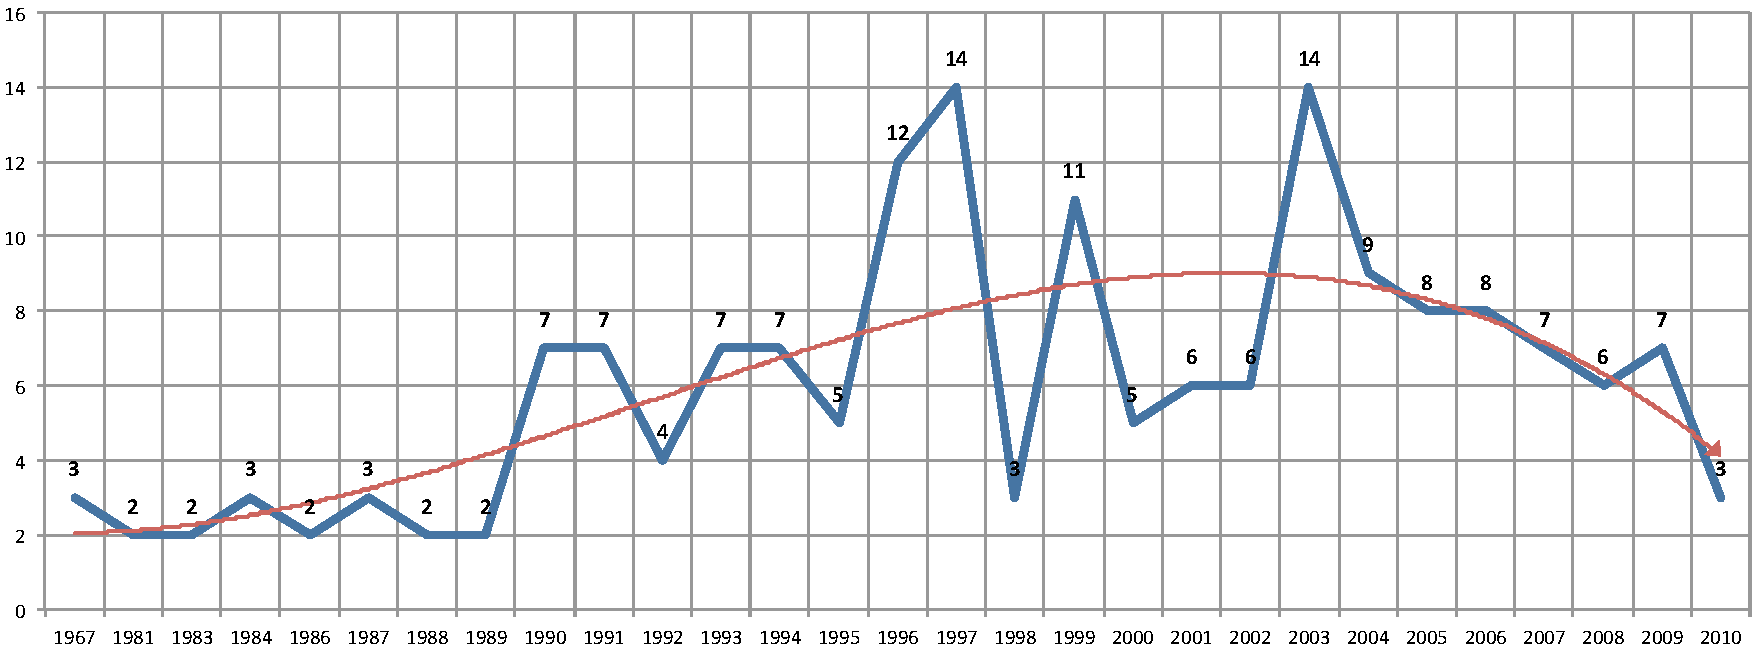
\includegraphics[scale=0.5]{imagens/abntex2-modelo-img-grafico.pdf}
	\end{center}
	\legend{Fonte: \citeonline[p. 24]{araujo2012}}
\end{figure}

% ---
\subsection{Figuras em \emph{minipages}}
% ---

\emph{Minipages} são usadas para inserir textos ou outros elementos em quadros
com tamanhos e posições controladas. Veja o exemplo da
\autoref{fig_minipage_imagem1} e da \autoref{fig_minipage_grafico2}.

\begin{figure}[htb]
 \label{teste}
 \centering
  \begin{minipage}{0.4\textwidth}
    \centering
    \caption{Imagem 1 da minipage} \label{fig_minipage_imagem1}
    
\includegraphics[scale=0.9]{imagens/abntex2-modelo-img-marca.pdf}
    \legend{Fonte: Produzido pelos autores}
  \end{minipage}
  \hfill
  \begin{minipage}{0.4\textwidth}
    \centering
    \caption{Grafico 2 da minipage} \label{fig_minipage_grafico2}
    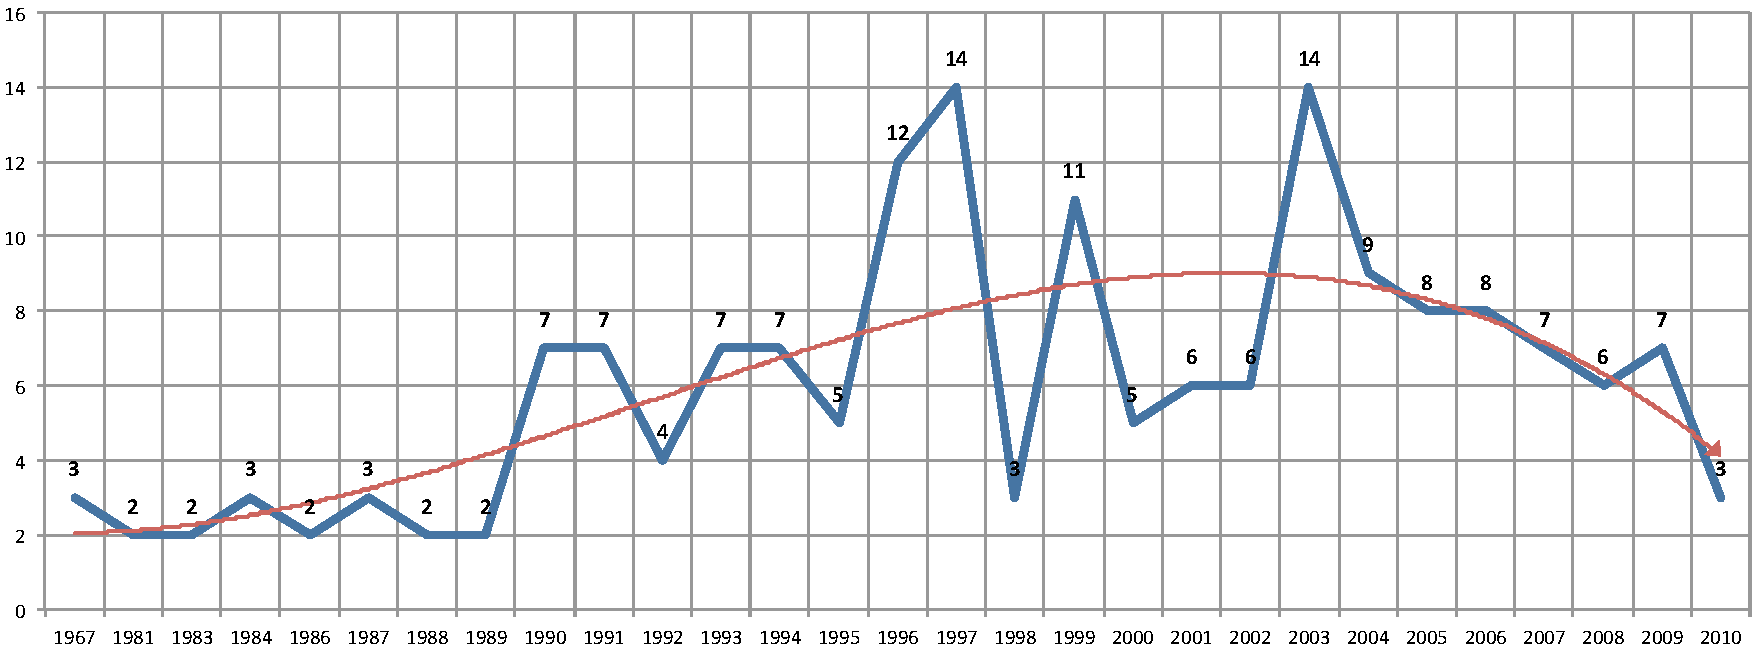
\includegraphics[scale=0.2]{imagens/abntex2-modelo-img-grafico.pdf}
    \legend{Fonte: \citeonline[p. 24]{araujo2012}}
  \end{minipage}
\end{figure}

Observe que, segundo a \citeonline[seções 4.2.1.10 e 5.8]{NBR14724:2011}, as
ilustrações devem sempre ter numeração contínua e única em todo o documento:

\begin{citacao}
Qualquer que seja o tipo de ilustração, sua identificação aparece na parte
superior, precedida da palavra designativa (desenho, esquema, fluxograma,
fotografia, gráfico, mapa, organograma, planta, quadro, retrato, figura,
imagem, entre outros), seguida de seu número de ordem de ocorrência no texto,
em algarismos arábicos, travessão e do respectivo título. Após a ilustração, na
parte inferior, indicar a fonte consultada (elemento obrigatório, mesmo que
seja produção do próprio autor), legenda, notas e outras informações
necessárias à sua compreensão (se houver). A ilustração deve ser citada no
texto e inserida o mais próximo possível do trecho a que se
refere. \cite[seções 5.8]{NBR14724:2011}
\end{citacao}

% % ---
% \section{Expressões matemáticas}
% % ---

% \index{expressões matemáticas}Use o ambiente \texttt{equation} para escrever
% expressões matemáticas numeradas:

% \begin{equation}
%   \forall x \in X, \quad \exists \: y \leq \epsilon
% \end{equation}

% Escreva expressões matemáticas entre \$ e \$, como em $ \lim_{x \to \infty}
% \exp(-x) = 0 $, para que fiquem na mesma linha.

% Também é possível usar colchetes para indicar o início de uma expressão
% matemática que não é numerada.

% \[
% \left|\sum_{i=1}^n a_ib_i\right|
% \le
% \left(\sum_{i=1}^n a_i^2\right)^{1/2}
% \left(\sum_{i=1}^n b_i^2\right)^{1/2}
% \]

% Consulte mais informações sobre expressões matemáticas em
% \url{https://github.com/abntex/abntex2/wiki/Referencias}.

% % ---
% \section{Enumerações: alíneas e subalíneas}
% % ---

% \index{alíneas}\index{subalíneas}\index{incisos}Quando for necessário enumerar
% os diversos assuntos de uma seção que não possua título, esta deve ser
% subdividida em alíneas \cite[4.2]{NBR6024:2012}:

% \begin{alineas}

%   \item os diversos assuntos que não possuam título próprio, dentro de uma mesma
%   seção, devem ser subdivididos em alíneas; 
  
%   \item o texto que antecede as alíneas termina em dois pontos;
%   \item as alíneas devem ser indicadas alfabeticamente, em letra minúscula,
%   seguida de parêntese. Utilizam-se letras dobradas, quando esgotadas as
%   letras do alfabeto;

%   \item as letras indicativas das alíneas devem apresentar recuo em relação à
%   margem esquerda;

%   \item o texto da alínea deve começar por letra minúscula e terminar em
%   ponto-e-vírgula, exceto a última alínea que termina em ponto final;

%   \item o texto da alínea deve terminar em dois pontos, se houver subalínea;

%   \item a segunda e as seguintes linhas do texto da alínea começa sob a
%   primeira letra do texto da própria alínea;
  
%   \item subalíneas \cite[4.3]{NBR6024:2012} devem ser conforme as alíneas a
%   seguir:

%   \begin{alineas}
%      \item as subalíneas devem começar por travessão seguido de espaço;

%      \item as subalíneas devem apresentar recuo em relação à alínea;

%      \item o texto da subalínea deve começar por letra minúscula e terminar em
%      ponto-e-vírgula. A última subalínea deve terminar em ponto final, se não
%      houver alínea subsequente;

%      \item a segunda e as seguintes linhas do texto da subalínea começam sob a
%      primeira letra do texto da própria subalínea.
%   \end{alineas}
  
%   \item no \abnTeX\ estão disponíveis os ambientes \texttt{incisos} e
%   \texttt{subalineas}, que em suma são o mesmo que se criar outro nível de
%   \texttt{alineas}, como nos exemplos à seguir:
  
%   \begin{incisos}
%     \item \textit{Um novo inciso em itálico};
%   \end{incisos}
  
%   \item Alínea em \textbf{negrito}:
  
%   \begin{subalineas}
%     \item \textit{Uma subalínea em itálico};
%     \item \underline{\textit{Uma subalínea em itálico e sublinhado}}; 
%   \end{subalineas}
  
%   \item Última alínea com \emph{ênfase}.
  
% \end{alineas}

% % ---
% \section{Espaçamento entre parágrafos e linhas}
% % ---

% \index{espaçamento!dos parágrafos}O tamanho do parágrafo, espaço entre a margem
% e o início da frase do parágrafo, é definido por:

% \begin{verbatim}
%    \setlength{\parindent}{1.3cm}
% \end{verbatim}

% \index{espaçamento!do primeiro parágrafo}Por padrão, não há espaçamento no
% primeiro parágrafo de cada início de divisão do documento
% (\autoref{sec-divisoes}). Porém, você pode definir que o primeiro parágrafo
% também seja indentado, como é o caso deste documento. Para isso, apenas inclua o
% pacote \textsf{indentfirst} no preâmbulo do documento:

% \begin{verbatim}
%    \usepackage{indentfirst}      % Indenta o primeiro parágrafo de cada seção.
% \end{verbatim}

% \index{espaçamento!entre os parágrafos}O espaçamento entre um parágrafo e outro
% pode ser controlado por meio do comando:

% \begin{verbatim}
%   \setlength{\parskip}{0.2cm}  % tente também \onelineskip
% \end{verbatim}

% \index{espaçamento!entre as linhas}O controle do espaçamento entre linhas é
% definido por:

% \begin{verbatim}
%   \OnehalfSpacing       % espaçamento um e meio (padrão); 
%   \DoubleSpacing        % espaçamento duplo
%   \SingleSpacing        % espaçamento simples	
% \end{verbatim}

% Para isso, também estão disponíveis os ambientes:

% \begin{verbatim}
%   \begin{SingleSpace} ...\end{SingleSpace}
%   \begin{Spacing}{hfactori} ... \end{Spacing}
%   \begin{OnehalfSpace} ... \end{OnehalfSpace}
%   \begin{OnehalfSpace*} ... \end{OnehalfSpace*}
%   \begin{DoubleSpace} ... \end{DoubleSpace}
%   \begin{DoubleSpace*} ... \end{DoubleSpace*} 
% \end{verbatim}

% Para mais informações, consulte \citeonline[p. 47-52 e 135]{memoir}.

% % ---
% \section{Inclusão de outros arquivos}\label{sec-include}
% % ---

% É uma boa prática dividir o seu documento em diversos arquivos, e não
% apenas escrever tudo em um único. Esse recurso foi utilizado neste
% documento. Para incluir diferentes arquivos em um arquivo principal,
% de modo que cada arquivo incluído fique em uma página diferente, utilize o
% comando:

% \begin{verbatim}
%    \include{documento-a-ser-incluido}      % sem a extensão .tex
% \end{verbatim}

% Para incluir documentos sem quebra de páginas, utilize:

% \begin{verbatim}
%    \input{documento-a-ser-incluido}      % sem a extensão .tex
% \end{verbatim}

% % ---
% \section{Compilar o documento \LaTeX}
% % ---

% Geralmente os editores \LaTeX, como o
% TeXlipse\footnote{\url{http://texlipse.sourceforge.net/}}, o
% Texmaker\footnote{\url{http://www.xm1math.net/texmaker/}}, entre outros,
% compilam os documentos automaticamente, de modo que você não precisa se
% preocupar com isso.

% No entanto, você pode compilar os documentos \LaTeX usando os seguintes
% comandos, que devem ser digitados no \emph{Prompt de Comandos} do Windows ou no
% \emph{Terminal} do Mac ou do Linux:

% \begin{verbatim}
%    pdflatex ARQUIVO_PRINCIPAL.tex
%    bibtex ARQUIVO_PRINCIPAL.aux
%    makeindex ARQUIVO_PRINCIPAL.idx 
%    makeindex ARQUIVO_PRINCIPAL.nlo -s nomencl.ist -o ARQUIVO_PRINCIPAL.nls
%    pdflatex ARQUIVO_PRINCIPAL.tex
%    pdflatex ARQUIVO_PRINCIPAL.tex
% \end{verbatim}

% % ---
% \section{Remissões internas}
% % ---

% Ao nomear a \autoref{tab-nivinv} e a \autoref{fig_circulo}, apresentamos um
% exemplo de remissão interna, que também pode ser feita quando indicamos o
% \autoref{cap_exemplos}, que tem o nome \emph{\nameref{cap_exemplos}}. O número
% do capítulo indicado é \ref{cap_exemplos}, que se inicia à
% \autopageref{cap_exemplos}\footnote{O número da página de uma remissão pode ser
% obtida também assim:
% \pageref{cap_exemplos}.}.
% Veja a \autoref{sec-divisoes} para outros exemplos de remissões internas entre
% seções, subseções e subsubseções.

% O código usado para produzir o texto desta seção é:

% \begin{verbatim}
% Ao nomear a \autoref{tab-nivinv} e a \autoref{fig_circulo}, apresentamos um
% exemplo de remissão interna, que também pode ser feita quando indicamos o
% \autoref{cap_exemplos}, que tem o nome \emph{\nameref{cap_exemplos}}. O número
% do capítulo indicado é \ref{cap_exemplos}, que se inicia à
% \autopageref{cap_exemplos}\footnote{O número da página de uma remissão pode ser
% obtida também assim:
% \pageref{cap_exemplos}.}.
% Veja a \autoref{sec-divisoes} para outros exemplos de remissões internas entre
% seções, subseções e subsubseções.
% \end{verbatim}

% % ---
% \section{Divisões do documento: seção}\label{sec-divisoes}
% % ---

% Esta seção testa o uso de divisões de documentos. Esta é a
% \autoref{sec-divisoes}. Veja a \autoref{sec-divisoes-subsection}.

% \subsection{Divisões do documento: subseção}\label{sec-divisoes-subsection}

% Isto é uma subseção. Veja a \autoref{sec-divisoes-subsubsection}, que é uma
% \texttt{subsubsection} do \LaTeX, mas é impressa chamada de ``subseção'' porque
% no Português não temos a palavra ``subsubseção''.

% \subsubsection{Divisões do documento: subsubseção}
% \label{sec-divisoes-subsubsection}

% Isto é uma subsubseção.

% \subsubsection{Divisões do documento: subsubseção}

% Isto é outra subsubseção.

% \subsection{Divisões do documento: subseção}\label{sec-exemplo-subsec}

% Isto é uma subseção.

% \subsubsection{Divisões do documento: subsubseção}

% Isto é mais uma subsubseção da \autoref{sec-exemplo-subsec}.


% \subsubsubsection{Esta é uma subseção de quinto
% nível}\label{sec-exemplo-subsubsubsection}

% Esta é uma seção de quinto nível. Ela é produzida com o seguinte comando:

% \begin{verbatim}
% \subsubsubsection{Esta é uma subseção de quinto
% nível}\label{sec-exemplo-subsubsubsection}
% \end{verbatim}

% \subsubsubsection{Esta é outra subseção de quinto nível}\label{sec-exemplo-subsubsubsection-outro}

% Esta é outra seção de quinto nível.


% \paragraph{Este é um parágrafo numerado}\label{sec-exemplo-paragrafo}

% Este é um exemplo de parágrafo nomeado. Ele é produzida com o comando de
% parágrafo:

% \begin{verbatim}
% \paragraph{Este é um parágrafo nomeado}\label{sec-exemplo-paragrafo}
% \end{verbatim}

% A numeração entre parágrafos numeradaos e subsubsubseções são contínuas.

% \paragraph{Esta é outro parágrafo numerado}\label{sec-exemplo-paragrafo-outro}

% Esta é outro parágrafo nomeado.

% % ---
% \section{Este é um exemplo de nome de seção longo. Ele deve estar
% alinhado à esquerda e a segunda e demais linhas devem iniciar logo abaixo da
% primeira palavra da primeira linha}
% % ---

% Isso atende à norma \citeonline[seções de 5.2.2 a 5.2.4]{NBR14724:2011} 
%  e \citeonline[seções de 3.1 a 3.8]{NBR6024:2012}.

% % ---
% \section{Diferentes idiomas e hifenizações}
% \label{sec-hifenizacao}
% % ---

% Para usar hifenizações de diferentes idiomas, inclua nas opções do documento o
% nome dos idiomas que o seu texto contém. Por exemplo (para melhor
% visualização, as opções foram quebras em diferentes linhas):

% \begin{verbatim}
% \documentclass[
% 	12pt,
% 	openright,
% 	twoside,
% 	a4paper,
% 	english,
% 	french,
% 	spanish,
% 	brazil
% 	]{abntex2}
% \end{verbatim}

% O idioma português-brasileiro (\texttt{brazil}) é incluído automaticamente pela
% classe \textsf{abntex2}. Porém, mesmo assim a opção \texttt{brazil} deve ser
% informada como a última opção da classe para que todos os pacotes reconheçam o
% idioma. Vale ressaltar que a última opção de idioma é a utilizada por padrão no
% documento. Desse modo, caso deseje escrever um texto em inglês que tenha
% citações em português e em francês, você deveria usar o preâmbulo como abaixo:

% \begin{verbatim}
% \documentclass[
% 	12pt,
% 	openright,
% 	twoside,
% 	a4paper,
% 	french,
% 	brazil,
% 	english
% 	]{abntex2}
% \end{verbatim}

% A lista completa de idiomas suportados, bem como outras opções de hifenização,
% estão disponíveis em \citeonline[p.~5-6]{babel}.

% Exemplo de hifenização em inglês\footnote{Extraído de:
% \url{http://en.wikibooks.org/wiki/LaTeX/Internationalization}}:

% \begin{otherlanguage*}{english}
% \textit{Text in English language. This environment switches all language-related
% definitions, like the language specific names for figures, tables etc. to the other
% language. The starred version of this environment typesets the main text
% according to the rules of the other language, but keeps the language specific
% string for ancillary things like figures, in the main language of the document.
% The environment hyphenrules switches only the hyphenation patterns used; it can
% also be used to disallow hyphenation by using the language name
% `nohyphenation'.}
% \end{otherlanguage*}

% Exemplo de hifenização em francês\footnote{Extraído de:
% \url{http://bigbrowser.blog.lemonde.fr/2013/02/17/tu-ne-tweeteras-point-le-vatican-interdit-aux-cardinaux-de-tweeter-pendant-le-conclave/}}:

% \begin{otherlanguage*}{french}
% \textit{Texte en français. Pas question que Twitter ne vienne faire une
% concurrence déloyale à la traditionnelle fumée blanche qui marque l'élection
% d'un nouveau pape. Pour éviter toute fuite précoce, le Vatican a donc pris un
% peu d'avance, et a déjà interdit aux cardinaux qui prendront part au vote
% d'utiliser le réseau social, selon Catholic News Service. Une mesure valable
% surtout pour les neuf cardinaux – sur les 117 du conclave – pratiquants très
% actifs de Twitter, qui auront interdiction pendant toute la période de se
% connecter à leur compte.}
% \end{otherlanguage*}

% Pequeno texto em espanhol\footnote{Extraído de:
% \url{http://internacional.elpais.com/internacional/2013/02/17/actualidad/1361102009_913423.html}}:

% \foreignlanguage{spanish}{\textit{Decenas de miles de personas ovacionan al pontífice en su
% penúltimo ángelus dominical, el primero desde que anunciase su renuncia. El Papa se
% centra en la crítica al materialismo}}.

% O idioma geral do texto por ser alterado como no exemplo seguinte:

% \begin{verbatim}
%   \selectlanguage{english}
% \end{verbatim}

% Isso altera automaticamente a hifenização e todos os nomes constantes de
% referências do documento para o idioma inglês. Consulte o manual da classe
% \cite{abntex2classe} para obter orientações adicionais sobre internacionalização de
% documentos produzidos com \abnTeX.

% A \autoref{sec-citacao} descreve o ambiente \texttt{citacao} que pode receber
% como parâmetro um idioma a ser usado na citação.

% % ---
% \section{Consulte o manual da classe \textsf{abntex2}}
% % ---

% Consulte o manual da classe \textsf{abntex2} \cite{abntex2classe} para uma
% referência completa das macros e ambientes disponíveis. 

% Além disso, o manual possui informações adicionais sobre as normas ABNT
% observadas pelo \abnTeX\ e considerações sobre eventuais requisitos específicos
% não atendidos, como o caso da \citeonline[seção 5.2.2]{NBR14724:2011}, que
% especifica o espaçamento entre os capítulos e o início do texto, regra
% propositalmente não atendida pelo presente modelo.

% % ---
% \section{Referências bibliográficas}
% % ---

% A formatação das referências bibliográficas conforme as regras da ABNT são um
% dos principais objetivos do \abnTeX. Consulte os manuais
% \citeonline{abntex2cite} e \citeonline{abntex2cite-alf} para obter informações
% sobre como utilizar as referências bibliográficas.

% %-
% \subsection{Acentuação de referências bibliográficas}
% %-

% Normalmente não há problemas em usar caracteres acentuados em arquivos
% bibliográficos (\texttt{*.bib}). Porém, como as regras da ABNT fazem uso quase
% abusivo da conversão para letras maiúsculas, é preciso observar o modo como se
% escreve os nomes dos autores. Na ~\autoref{tabela-acentos} você encontra alguns
% exemplos das conversões mais importantes. Preste atenção especial para `ç' e `í'
% que devem estar envoltos em chaves. A regra geral é sempre usar a acentuação
% neste modo quando houver conversão para letras maiúsculas.

% \begin{table}[htbp]
% \caption{Tabela de conversão de acentuação.}
% \label{tabela-acentos}

% \begin{center}
% \begin{tabular}{ll}\hline\hline
% acento & \textsf{bibtex}\\
% à á ã & \verb+\`a+ \verb+\'a+ \verb+\~a+\\
% í & \verb+{\'\i}+\\
% ç & \verb+{\c c}+\\
% \hline\hline
% \end{tabular}
% \end{center}
% \end{table}


% % ---
% \section{Precisa de ajuda?}
% % ---

% Consulte a FAQ com perguntas frequentes e comuns no portal do \abnTeX:
% \url{https://github.com/abntex/abntex2/wiki/FAQ}.

% Inscreva-se no grupo de usuários \LaTeX:
% \url{http://groups.google.com/group/latex-br}, tire suas dúvidas e ajude
% outros usuários.

% Participe também do grupo de desenvolvedores do \abnTeX:
% \url{http://groups.google.com/group/abntex2} e faça sua contribuição à
% ferramenta.

% % ---
% \section{Você pode ajudar?}
% % ---

% Sua contribuição é muito importante! Você pode ajudar na divulgação, no
% desenvolvimento e de várias outras formas. Veja como contribuir com o \abnTeX\
% em \url{https://github.com/abntex/abntex2/wiki/Como-Contribuir}.

% % ---
% \section{Quer customizar os modelos do \abnTeX\ para sua instituição ou
% universidade?}
% % ---

% Veja como customizar o \abnTeX\ em:
% \url{https://github.com/abntex/abntex2/wiki/ComoCustomizar}.


% ---
% ---
% Capitulo 2
% ---
\chapter{Trabalhos Relacionados}
% ---
% ---esta seção, são exploradas pesquisas que compartilham afinidades e características semelhantes com os sistemas que este projeto busca desenvolver
Nesta seção, são exploradas pesquisas que compartilham afinidades e características semelhantes com o sistema que este projeto busca desenvolver

\section{TAF- teste de aptidão física da brigada militar do rio grande do sul}
Um aplicativo móvel que visa facilitar a aplicação e avaliação do TAF na brigada militar do rio grande do sul. 
O TAF tem como objetivo verificar se os candidatos possuem as condições físicas mínimas exigidas para desempenhar as atividades do cargo.\citeonline{taf}

O aplicativo foi desenvolvido em parceria do IFRS com a BM RS,proporcionando mais projetos como este para alunos da instituição e trazendo benefícios para órgãos governamentais, fortalecendo a integração prática do conhecimento acadêmico com as demandas da sociedade.

Na \autoref{fig:grafico-taf} é demonstrado a tela inicial do TAF

\begin{figure}[htb]
    \caption{\label{fig:grafico-taf}Tela Inicial do aplicativo TAF BM}
    \begin{center}
        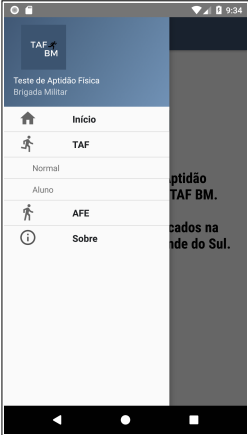
\includegraphics[scale=0.9]{imagens/taf.png}
    \end{center}
    \legend{Fonte: \citeonline{taf}}
\end{figure}
Por se tratar de resoluções em contextos diferentes, o aplicativo ''TAF'' se encaixa nesta seção por ter sido desenvolvido para a Brigada Militar do Rio Grande do Sul.   

\section{APLICATIVO WEB PARA PESSOAS FÍSICAS QUE UTILIZAM PRODUTOS CONTROLADOS PELO EXÉRCITO
BRASILEIRO E POLÍCIA FEDERAL}
A aplicação web denominada CRPG, tem o intuito de auxiliar os os usuários a lidar com as etapas necessárias para a aquisição de produtos controlados pelo Exército Brasileiro e Polícia Federal. A \autoref{fig:grafico-crpg} demonstra a tela de cadastro de processos:

\begin{figure}[htb]
    \caption{\label{fig:grafico-crpg}Tela de cadastros da aplicação CRPG}
    \begin{center}
        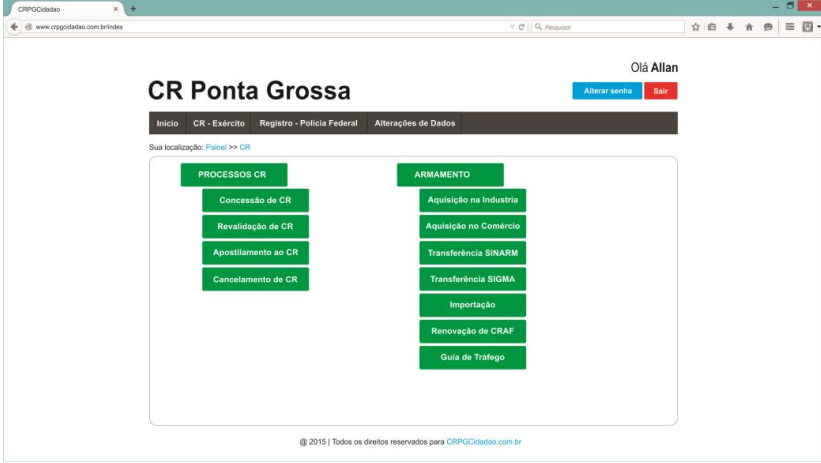
\includegraphics[scale=0.9]{imagens/crpg.png}
    \end{center}
    \legend{Fonte: \citeonline{crpg}}
\end{figure}

O Trabalho proposto se distingue da aplicação demonstrada acima, pois atua no âmbito de auxiliar os operadores da brigada militar afim de promover uma maior agilidade no processo de envio das informações para o SIGMA, buscando promover uma maior fluidez no controle e regulamentação dos produtos controlados sob jurisdição do exercito que estão sob posse destes indivíduos e entidades mencionadas na \autoref{sigmaesinarm}



\section{SISTEMA DE GERENCIAMENTO DE LICENÇAS DE POSSE E PORTE DE ARMAS DE FOGO}
Esta aplicação web se propõe a realizar todos os processos, como cadastro, validação de licenças, emissão de guias de tráfego, para indivíduos que tenham ou queiram adquirir o posse e porte de armas.

\begin{figure}[htb]
    \caption{\label{fig:grafico-sglppa} Tela de cadastros da aplicação de Gerenciamento de Licenças}
    \begin{center}
        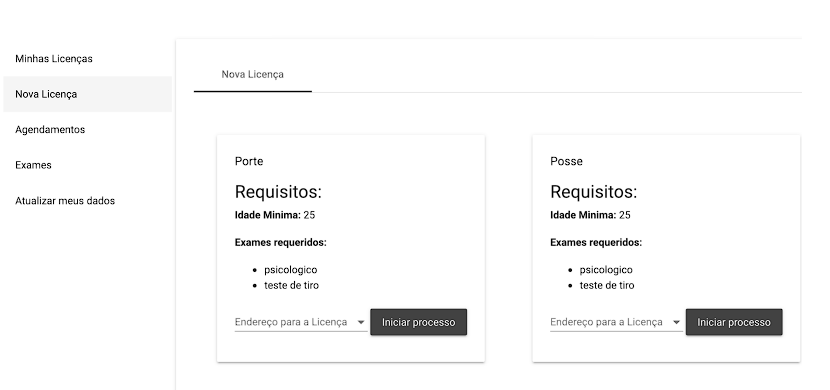
\includegraphics[scale=0.8]{imagens/sglppa.png}
    \end{center}
    \legend{Fonte: \citeonline{sglppa}}
\end{figure}

O presente trabalho destaca-se da aplicação anterior ao concentrar seus esforços na assistência aos operadores da brigada militar, visando agilizar o envio de informações para o SIGMA. A intenção é favorecer uma maior fluidez no controle e regulamentação desses produtos controlados sob jurisdição do exército.


% ---

% ---
% Capitulo 3
% ---
\chapter{Metodologia}
% ---
% ---
Neste segmento, serão delineadas informações relacionadas à elaboração da aplicação proposta neste projeto. Discutiremos a estruturação do desenvolvimento e a análise de requisitos, abrangendo tanto os funcionais quanto os não funcionais.

Na delineação da Estruturação do desenvolvimento, é vital compreender a sinergia entre os componentes, visando otimizar a eficiência e a coesão do sistema em questão. Os requisitos funcionais, sendo pilares fundamentais, demandam uma abordagem analítica aprimorada para assegurar sua implementação fluída.

Quanto aos requisitos não funcionais, devemos explorar suas nuances de maneira minudente, reconhecendo a importância intrínseca de cada faceta no contexto global do projeto. Esta abordagem detalhada proporciona uma compreensão mais profunda, permitindo a delimitação precisa de parâmetros que transcendem as fronteiras meramente operacionais.

\section{Estruturação do desenvolvimento}\label{sec:estruturacao-desenvolvimento}
A forma como foi organizado o desenvolvimento do presente trabalho consiste inicialmente em pesquisas exploratórias realizadas através de entrevistas conduzidas com um membro da Brigada Militar, SD. Tiago Costa. Durante essas entrevistas, foram formuladas perguntas pertinentes ao procedimento de geração do AEL.

A coleta de informações foi complementada por meio de análise documental, sendo como principal embasamento a Portaria 136 de 8 de novembro de 2019 do Exército Brasileiro, mais especificamente o anexo D do \citeonline{ExércitoBrasileiro} constante nos Anexos (\ref{sec:anexoA1}, \ref{sec:anexoA2}, \ref{sec:anexoA3}, \ref{sec:anexoA4}). Esta documentação conceitua todas as fases envolvidas no processo de geração do AEL da Brigada Militar do Rio Grande do Sul.

A partir da análise de escopo realizada, planejou-se o uso do modelo de desenvolvimento iterativo neste projeto pois de acordo com \citeonline{engenhariasw}, se um processo interno de desenvolvimento iterativo é usado, o documento de requisitos pode ser muito menos detalhado e quaisquer ambiguidades podem ser resolvidas durante o desenvolvimento do sistema.

Logo a complexidade do procedimento de geração do AEL demanda uma abordagem flexível, permitindo ajustes contínuos à medida que novos pontos de vista são revelados durante entrevistas com SD. Tiago Costa. Essa metodologia proporciona validação incremental das fases, adaptabilidade a mudanças nos requisitos e envolvimento constante, garantindo um desenvolvimento mais preciso.


\section{Análise de Requisitos}
Os requisitos inerentes a aplicação web, foram levantados com base nas informações coletadas durantes as reuniões com os envolvidos conforme citado na \autoref{sec:estruturacao-desenvolvimento} sendo avaliado como as funcionalidades essenciais aquelas que impactam diretamente o pleno funcionamento da aplicação, quais devem ser implementadas durante o desenvolvimento do sistema. Ademais, foi realizada uma avaliação para determinar as funcionalidades desejáveis.

Sendo divida esta em subseções contendo os requisitos funcionais e não funcionais.

\subsection{Requisitos Funcionais}
Nesta subseção, será abordado os requisitos funcionais, aqueles que abrangem e descrevem todas as funcionalidades previstas para o sistema. 

\begin{table}[H]\label{tab:rf01}
    \caption{Requisito Funcional 1}
    \centering
    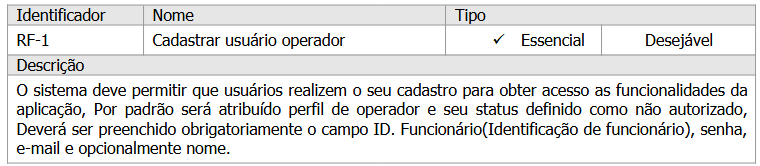
\includegraphics[scale=0.82]{imagens/rf01.png}
    \legend{Fonte: Autor}
\end{table}
\begin{table}[H]\label{tab:rf02}
    \caption{Requisito Funcional 2}
    \centering
    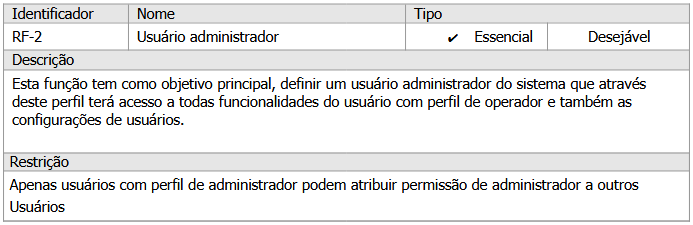
\includegraphics[scale=0.82]{imagens/rf02.png}
    \legend{Fonte: Autor}
\end{table}
\begin{table}[H]\label{tab:rf03}
    \caption{Requisito Funcional 3}
    \centering
    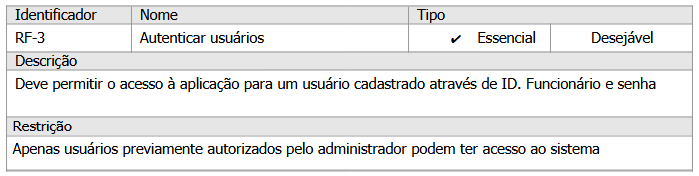
\includegraphics[scale=0.9]{imagens/rf03.png}
    \legend{Fonte: Autor}
\end{table}
\begin{table}[H]\label{tab:rf04}
    \caption{Requisito Funcional 4}
    \centering
    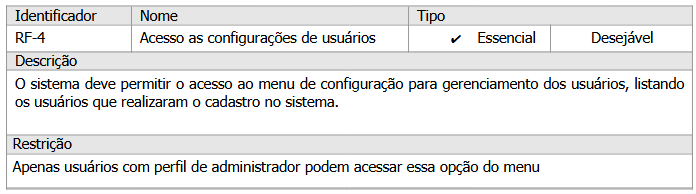
\includegraphics[scale=0.9]{imagens/rf04.png}
    \legend{Fonte: Autor}
\end{table}
\begin{table}[H]\label{tab:rf05}
    \caption{Requisito Funcional 5}
    \centering
    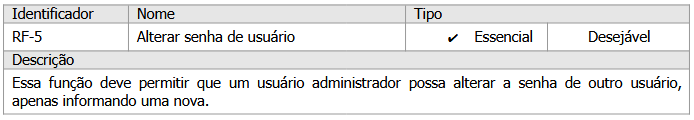
\includegraphics[scale=0.9]{imagens/rf05.png}
    \legend{Fonte: Autor}
\end{table}
\begin{table}[H]
    \caption{Requisito Funcional 6}\label{tab:rf06}
    \centering
    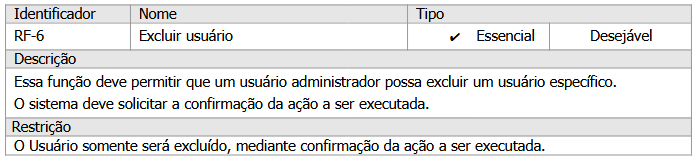
\includegraphics[scale=0.9]{imagens/rf06.png}
    \legend{Fonte: Autor}
\end{table}
\begin{table}[H]
    \caption{Requisito Funcional 7}\label{tab:rf07}
    \centering
    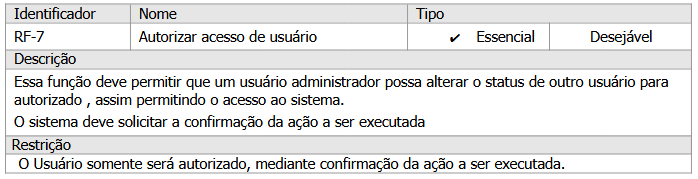
\includegraphics[scale=0.9]{imagens/rf07.png}
    \legend{Fonte: Autor}
\end{table}
\begin{table}[H]
    \caption{Requisito Funcional 8}\label{tab:rf08}
    \centering
    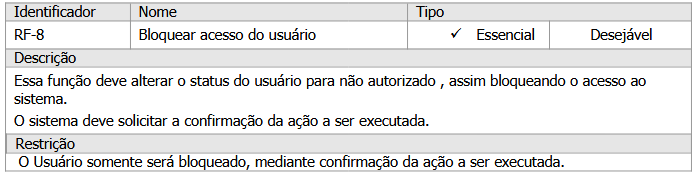
\includegraphics[scale=0.9]{imagens/rf08.png}
    \legend{Fonte: Autor}
\end{table}
\begin{table}[H]
    \caption{Requisito Funcional 9}\label{tab:rf09}
    \centering
    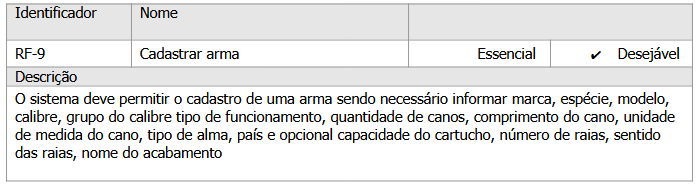
\includegraphics[scale=0.9]{imagens/rf09.png}
    \legend{Fonte: Autor}
\end{table}
\begin{table}[H]
    \caption{Requisito Funcional 10}\label{tab:rf10}
    \centering
    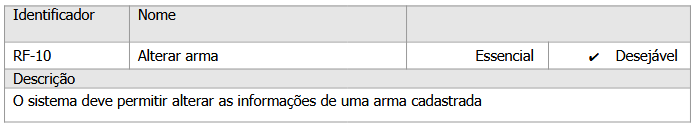
\includegraphics[scale=0.9]{imagens/rf10.png}
    \legend{Fonte: Autor}
\end{table}
\begin{table}[H]
    \caption{Requisito Funcional 11}\label{tab:rf11}
    \centering
    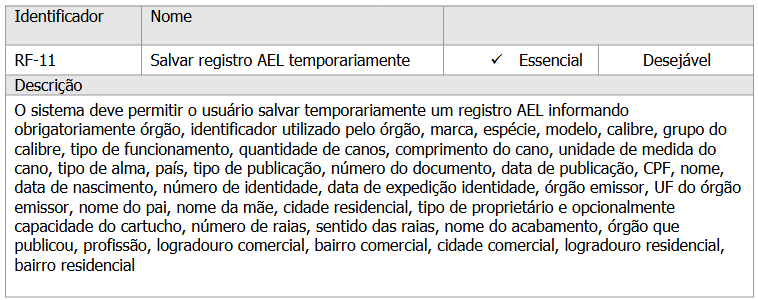
\includegraphics[scale=0.82]{imagens/rf11.png}
    \legend{Fonte: Autor}
\end{table}
\begin{table}[H]
    \caption{Requisito Funcional 12}\label{tab:rf12}
    \centering
    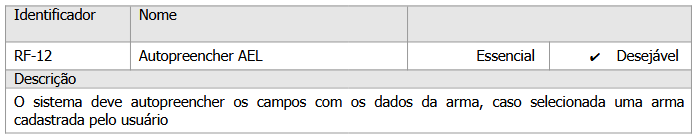
\includegraphics[scale=0.9]{imagens/rf12.png}
    \legend{Fonte: Autor}
\end{table}
\begin{table}[H]
    \caption{Requisito Funcional 13}\label{tab:rf13}
    \centering
    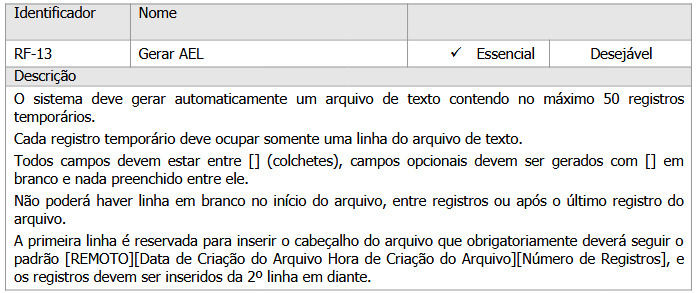
\includegraphics[scale=0.9]{imagens/rf13.png}
    \legend{Fonte: Autor}
\end{table}
\begin{table}[H]
    \caption{Requisito Funcional 14}\label{tab:rf14}
    \centering
    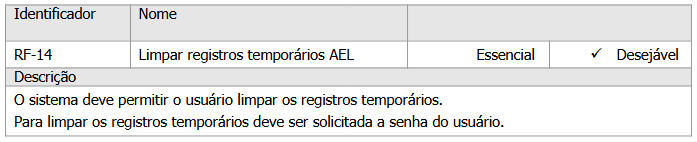
\includegraphics[scale=0.9]{imagens/rf14.png}
    \legend{Fonte: Autor}
\end{table}



\subsection{Requisitos Não Funcionais}
Na presente subseção, serão apresentados os requisitos não funcionais da aplicação, os quais descrevem as características globais do sistema, indo além das funcionalidades específicas.
E assegurando uma compreensão completa e abrangente dos métodos empregados pela aplicação para alcançar o resultado almejado.

\begin{table}[H]
    \caption{Requisito Não Funcional 1}\label{tab:rnf1}
    \centering
    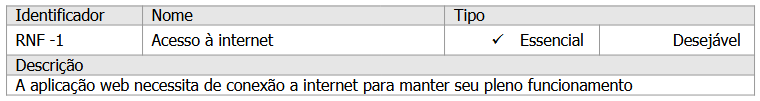
\includegraphics[scale=0.82]{imagens/rnf1.png}
    \legend{Fonte: Autor}
\end{table}
\begin{table}[H]
    \caption{Requisito Não Funcional 2}\label{tab:rnf2}
    \centering
    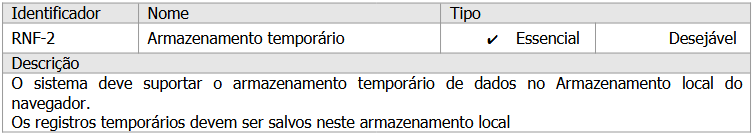
\includegraphics[scale=0.82]{imagens/rnf2.png}
    \legend{Fonte: Autor}
\end{table}
\begin{table}[H]
    \caption{Requisito Não Funcional 3}\label{tab:rnf3}
    \centering
    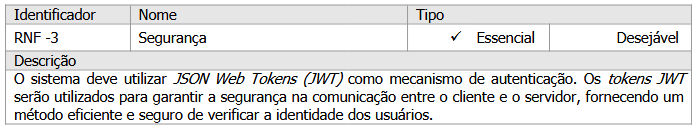
\includegraphics[scale=0.82]{imagens/rnf3.png}
    \legend{Fonte: Autor}
\end{table}
\begin{table}[H]
    \caption{Requisito Não Funcional 4}\label{tab:rnf4}
    \centering
    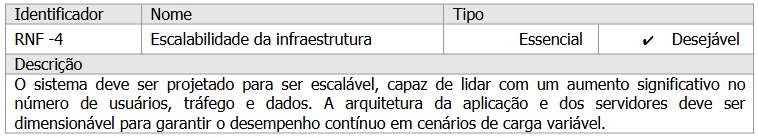
\includegraphics[scale=0.82]{imagens/rnf4.png}
    \legend{Fonte: Autor}
\end{table}
\begin{table}[H]
    \caption{Requisito Não Funcional 5}\label{tab:rnf5}
    \centering
    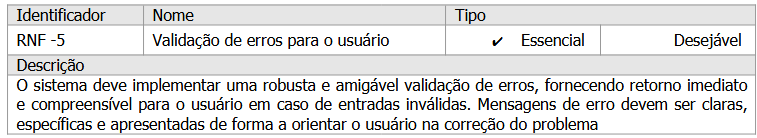
\includegraphics[scale=0.82]{imagens/rnf5.png}
    \legend{Fonte: Autor}
\end{table}
\begin{table}[H]
    \caption{Requisito Não Funcional 6}\label{tab:rnf6}
    \centering
    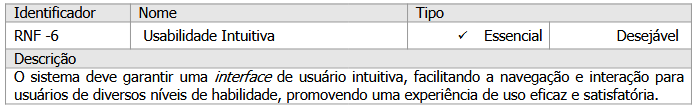
\includegraphics[scale=0.82]{imagens/rnf6.png}
    \legend{Fonte: Autor}
\end{table}
% % ---
% \section{Tabelas}
% % ---

% \index{tabelas}A \autoref{tab-nivinv} é um exemplo de tabela construída em
% \LaTeX.

% \begin{table}[htb]
% \ABNTEXfontereduzida
% \caption[Níveis de investigação]{Níveis de investigação.}
% \label{tab-nivinv}
% \begin{tabular}{p{2.6cm}|p{6.0cm}|p{2.25cm}|p{3.40cm}}
%   %\hline
%    \textbf{Nível de Investigação} & \textbf{Insumos}  & \textbf{Sistemas de Investigação}  & \textbf{Produtos}  \\
%     \hline
%     Meta-nível & Filosofia\index{filosofia} da Ciência  & Epistemologia &
%     Paradigma  \\
%     \hline
%     Nível do objeto & Paradigmas do metanível e evidências do nível inferior &
%     Ciência  & Teorias e modelos \\
%     \hline
%     Nível inferior & Modelos e métodos do nível do objeto e problemas do nível inferior & Prática & Solução de problemas  \\
%    % \hline
% \end{tabular}
% \legend{Fonte: \citeonline{van86}}
% \end{table}

% Já a \autoref{tabela-ibge} apresenta uma tabela criada conforme o padrão do
% \citeonline{ibge1993} requerido pelas normas da ABNT para documentos técnicos e
% acadêmicos.

% \begin{table}[htb]
% \IBGEtab{%
%   \caption{Um Exemplo de tabela alinhada que pode ser longa
%   ou curta, conforme padrão IBGE.}%
%   \label{tabela-ibge}
% }{%
%   \begin{tabular}{ccc}
%   \toprule
%    Nome & Nascimento & Documento \\
%   \midrule \midrule
%    Maria da Silva & 11/11/1111 & 111.111.111-11 \\
%   \midrule 
%    João Souza & 11/11/2111 & 211.111.111-11 \\
%   \midrule 
%    Laura Vicuña & 05/04/1891 & 3111.111.111-11 \\
%   \bottomrule
% \end{tabular}%
% }{%
%   \fonte{Produzido pelos autores.}%
%   \nota{Esta é uma nota, que diz que os dados são baseados na
%   regressão linear.}%
%   \nota[Anotações]{Uma anotação adicional, que pode ser seguida de várias
%   outras.}%
%   }
% \end{table}
% ---



\chapter{Desenvolvimento da aplicação AutoForm}
% ---
Neste capitulo é apresentado o desenvolvimento do projeto, onde são apresentados,arquitetura do sistema,o processo de produção, e a implementação do sistema.

\subsection{Processo de produção}
O projeto teve sua fase inicial, após o 1º encontro com o cliente Tiago Costa e o coorientador Márcio Lemos no \textit{campus} Osório do IFRS, conforme demonstrado a necessidade pela BMRS de uma aplicação que pudesse ser utilizada para auxiliar no processo de registro do AEL no SIGMA, a fim de agilizar o processo de preenchimento e automatizar a geração do arquivo, bem como resolver outras dificuldades encontradas pelos operadores.
Após a definição de contexto do AEL por parte da BM RS, foi realizado um estudo sobre o assunto, para que fosse possível entender o problema e propor uma solução viável e eficaz. 

Com a elicitação dos requisitos concluída, ocorreu a prototipação das telas da aplicação, utilizando a ferramenta de \textit{design de interface } de usuário \cite{figma}, a fim de validar se o visual e o fluxo da aplicação iriam atender o proposito da instituição.

\subsubsection{Tecnologias}\label{sec:tecnologias}
Após a validação do protótipo, foi realizada a escolha das tecnologias que seriam utilizadas no desenvolvimento da aplicação, sendo elas o \textit{framework} \cite{React22:online}, para o desenvolvimento \textit{frontend}, e o \textit{framework} NodeJS \cite{Nodejs} para o desenvolvimento do \textit{backend} da aplicação web, juntamente com o banco de dados não relacional \cite{MongoDBA45:online}, para o armazenamento dos dados.

Com as tecnologias definidas, foi realizado o desenvolvimento da aplicação web e hospedado em um servidor, para que fosse possível realizar os testes e validações com o cliente, e assim, realizar as correções necessárias. 

Portanto após a primeira versão da aplicação estar disponível na \textit{internet} as adaptações necessárias e atualizações eram organizadas e relatadas mediante troca de mensagens com o cliente.

Para permitir que fosse possível realizar atualizações em produção na aplicação foi utilizada a ferramente\cite{git}, juntamente com a plataforma de hospedagem de código fonte \cite{github}, para que fosse possível realizar o controle de versões e o versionamento do código fonte da aplicação, garantindo sempre uma versão estável e disponivel em produção, enquanto era viável desenvolver paralelamente novas funcionalidades e valida-las com o cliente.

\subsection{Arquitetura da aplicação}
Nesta seção será abordado a visão de como foi projetado a estrutura do sistema que é composto por uma aplicação web, e uma API.

A Arquitetura \textit{MVC} foi a escolhida para a estruturação do sistema, ficando então dispostas as tecnologias mencionadas na \autoref{sec:tecnologias} da seguinte maneira ilustradas pela  \autoref{fig:diagramstacks}.

\begin{figure}[htb]
    \caption{\label{fig:diagramstacks}Disposição das tecnologias na arquitetura MVC}
    \begin{center}
        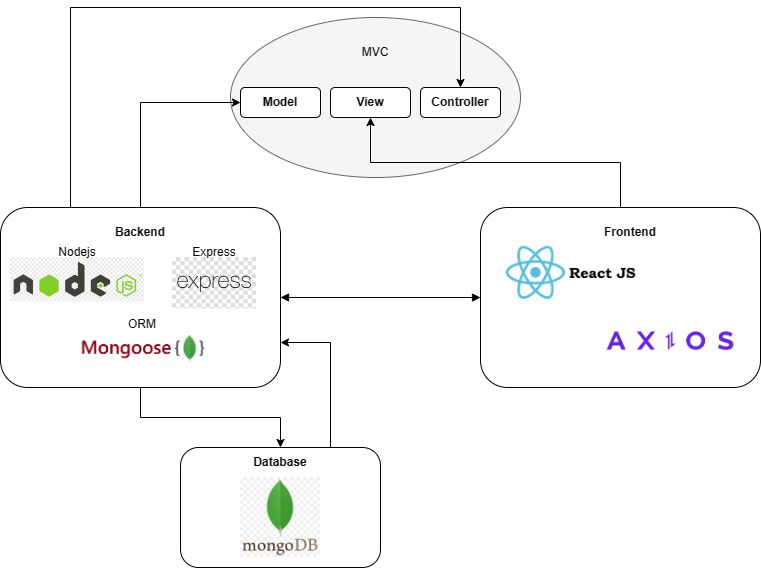
\includegraphics[scale=0.5]{imagens/diagrama.png}
    \end{center}
    \legend{Fonte: Autor}
\end{figure}


Toda comunicação entre a aplicação web e a API é realizada através de requisições HTTP, onde a aplicação web realiza requisições para a API, e a API responde com os dados solicitados, caso necessário a API busca as informações no banco de dados e retorna para a aplicação web.

As requisições e respostas seguem o padrão REST, onde cada requisição possui um método HTTP, e um \textit{endpoint} que é a URL que identifica o recurso que está sendo solicitado, e a resposta da requisição é um JSON, que contém os dados solicitados.



\subsection{Aplicação Web AutoForm}

\subsubsection{Autenticação}

A página para acessar a aplicação \autoref{fig:tela-login} e a página de registro \autoref{fig:tela-registro} são de acesso público, portanto podem ser visualizadas sem a necessidade de autenticação, já as demais páginas é necessário realizar o login.

A estratégia empregada para o acesso consiste na autenticação por meio de token JWT. O usuário realiza o login, fornecendo sua identificação de funcionário e senha. Essas informações são então encaminhadas para a API por meio de uma requisição POST. 
A API valida no banco de dados a existência de um usuário com os dados fornecidos. 
Se a validação for bem-sucedida, a API gera um token de acesso e o retorna como resposta. Posteriormente, a aplicação decodifica o token recebido, que contém as informações do usuário no \textit{payload}, e armazena os dados de identificação no navegador da pessoa que solicitou o acesso.

E a cada requisição posterior para outros \textit{endpoints} que a aplicação realize para a API, o token é enviado no cabeçalho da requisição,e a API irá validar somente o token, e caso seja válido retorna os dados solicitados.

\subsubsection{Página de login}
Está página é responsavel por realizar a autenticação do usuário, e para isso é necessário informar a identificação de funcionário e a senha, e caso o usuário não possua cadastro, é possível realizar o registro, clicando no botão "Registrar-se", que redireciona para a página de registro.

\begin{figure}[htb]
    \caption{\label{fig:tela-login}Autoform - Página de login}
    \begin{center}
        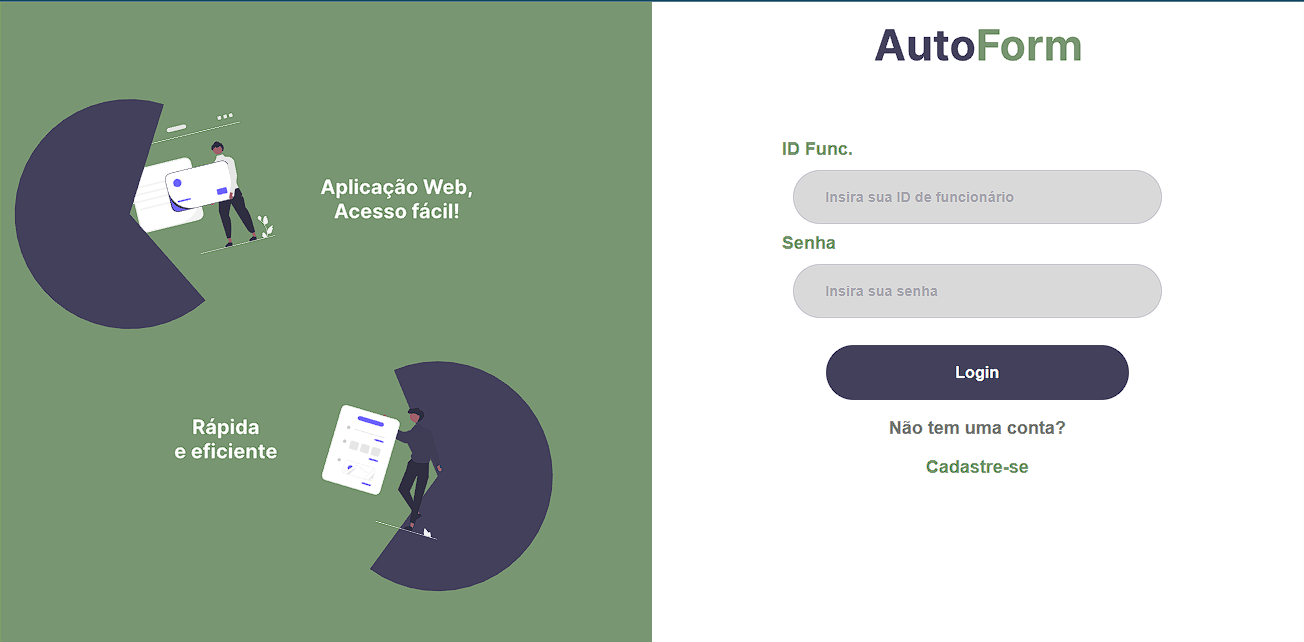
\includegraphics[scale=0.5]{imagens/login-autoform.png}
    \end{center}
    \legend{Fonte: Autor}
\end{figure}

 Se, por acaso, a validação no banco de dados não for bem-sucedida, a API emite uma resposta personalizada, indicando a natureza específica do impedimento.

Em um cenário em que a Identificação de Funcionário ou a senha fornecida não corresponde aos registros existentes, um alerta sutil é gerado, informando ao usuário sobre a disparidade. Este mecanismo proativo visa aprimorar a eficiência da correção do erro, direcionando o usuário a revisar e corrigir suas credenciais antes de prosseguir com a autenticação.
Ademais, é importante ressaltar que, em situações extremas, como indisponibilidade temporária do serviço de autenticação, o usuário é informado sobre a impossibilidade de acesso, e orientado a tentar novamente mais tarde.

\subsubsection{Página de registro}
A página de registro \autoref{fig:tela-registro} é responsável por realizar o cadastro de novos usuários, e para isso é necessário informar o email, a identificação de funcionário, a senha, e a confirmação da senha, em caso de sucesso será retornada uma mensagem informando que o registro foi efetuado com sucesso.

\begin{figure}[htb]
    \caption{\label{fig:tela-registro}Autoform - Página de registros}
    \begin{center}
        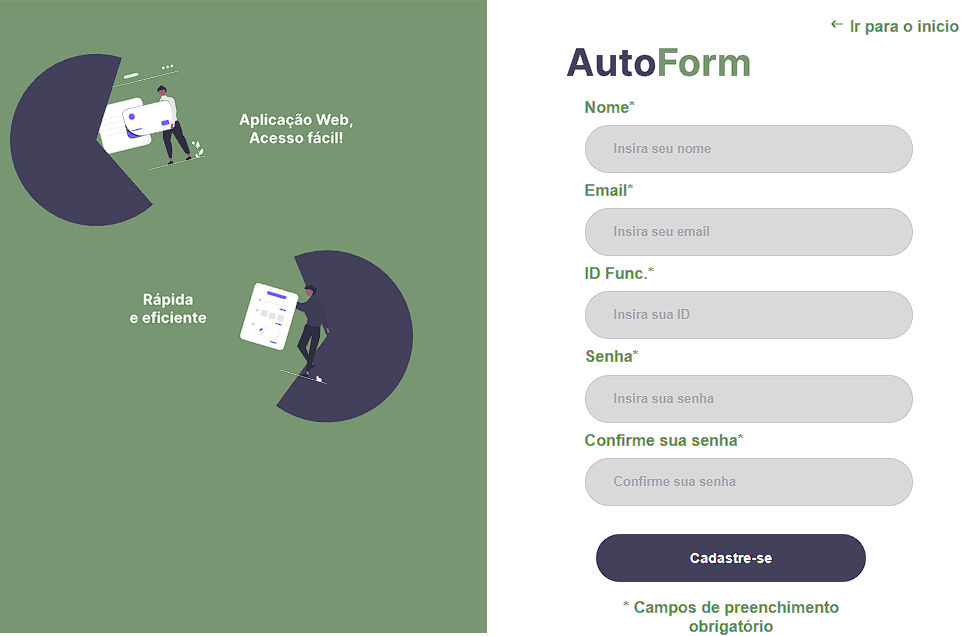
\includegraphics[scale=0.6]{imagens/registro-autoform.png}   
     \end{center}
    \legend{Fonte: Autor}
\end{figure}
Caso a identificação de funcionário já esteja cadastrada, será retornado uma mensagem informando que a identificação de funcionário já está cadastrada.
Em caso de não conformidade da senha com a confirmação da senha, será retornado uma mensagem informando que as senhas não conferem.

\subsubsection{Página inicial}
Esta é a página inicial da aplicação, a qual o usuário é direcionado assim que realiza o login, e nela é possível visualizar no menu lateral as opções disponíveis de criação de AEL, cadastros, e configurações.

\begin{figure}[htb]
    \caption{\label{fig:tela-home}Autoform - Página inicial home}
    \begin{center}
        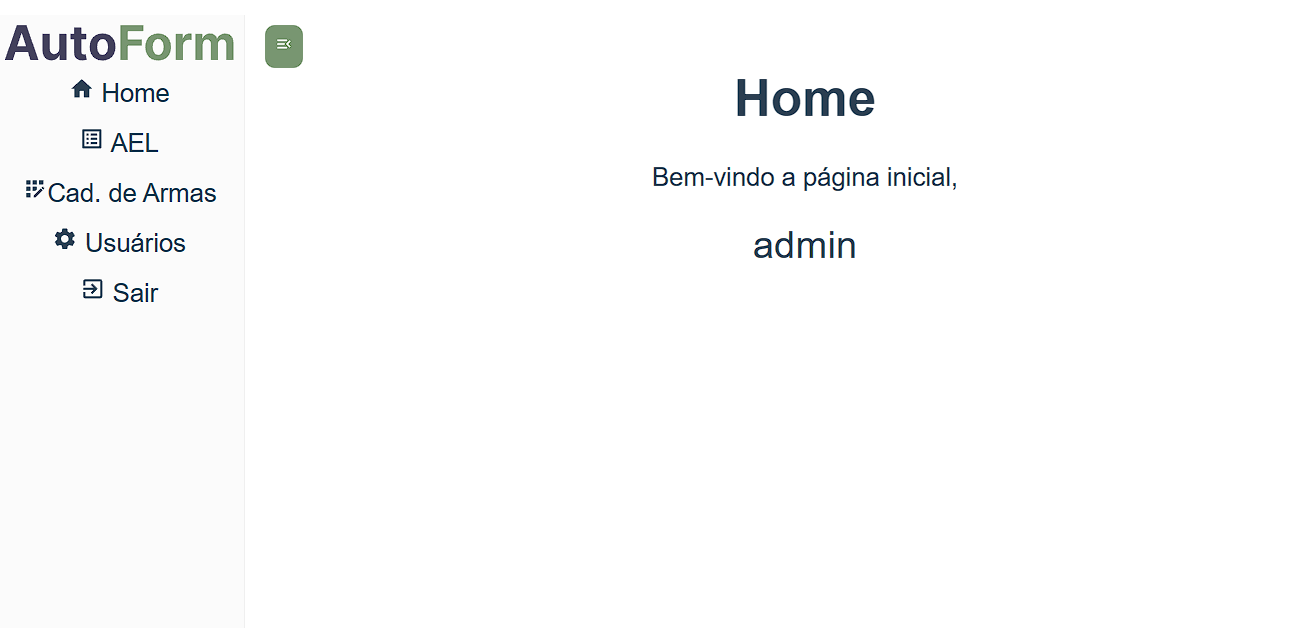
\includegraphics[scale=0.5]{imagens/home-autoform.png}
    \end{center}
    \legend{Fonte: Autor}
\end{figure}

\subsubsection{Página de criação de AEL}
A página de criação de AEL \autoref{fig:tela-ael1} é responsável por realizar a criação de um registro e geração do AEL, sendo necessário informar os campos obrigatórios que constam no \autoref{sec:anexoA2} e \autoref{sec:anexoA3}.

Cada registro é salvo no \textit{local storage} do navegador do usuário com todas informações preenchidas no formulário, para posterior geração do arquivo. 

Essa estrategia de armazenamento temporário foi adota visando manter a integridade e a segurança das informações caso o usuário perca a conexão com a internet ou por algum outro motivo a aplicação do navegador seja encerrada, acarretaria na perca de todos os registros já digitados, utilizando essa abordagem é possível resgatar da memoria do navegado todos os registros salvos temporariamente para geração do AEL, sem necessidade de armazenar no banco de dados ou enviar pela rede informações sensíveis como CPF entre outros. 
\begin{figure}[htb]
    \caption{\label{fig:tela-ael1}Autoform - Página criação AEL}
    \begin{center}
        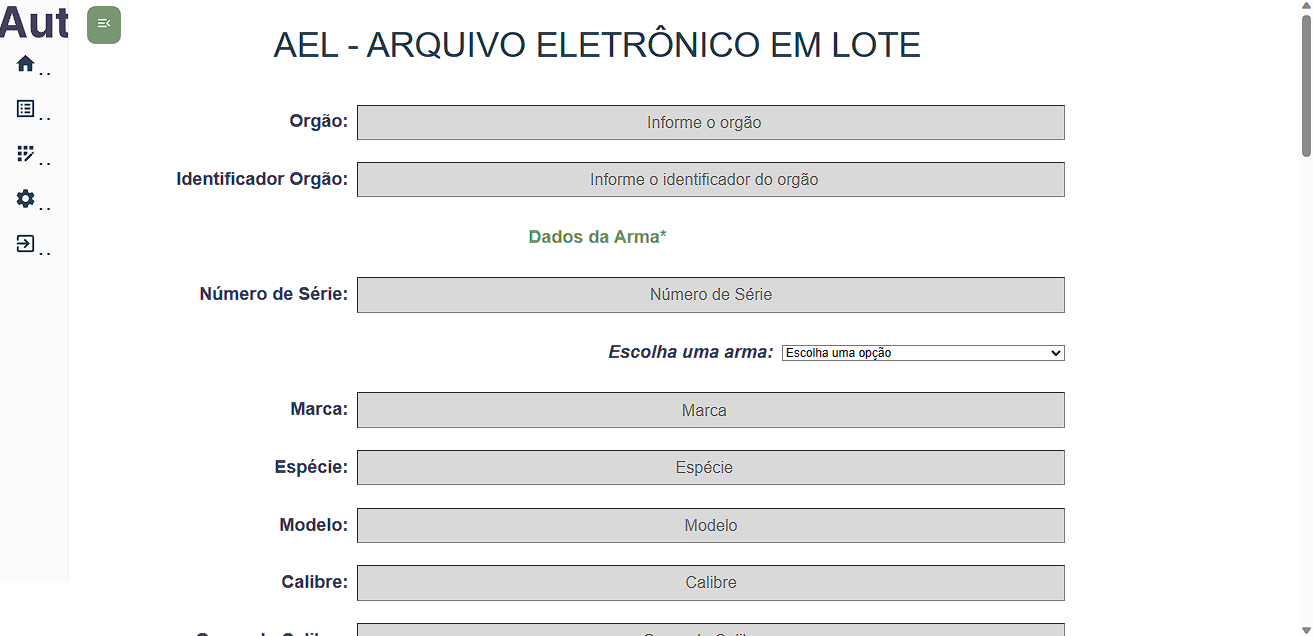
\includegraphics[scale=0.5]{imagens/autoform-ael-gerar.png}
    \end{center}
    \legend{Fonte: Autor}
\end{figure}

\subsubsection{Página de criação de AEL com opção de autopreenchimento}
Na \autoref{fig:tela-ael-selecao} podemos visualizar um input que exibe uma lista com as armas cadastradas, facilitando o preenchimento de diversos campos do formulário.
Pois permite o usuário selecionar uma arma já cadastrada, e os respectivos campos do formulário serão preenchidos automaticamente.

\begin{figure}[H]
    \caption{\label{fig:tela-ael-selecao}Autoform - Página criação AEL com opção para selecionar}
    \begin{center}
        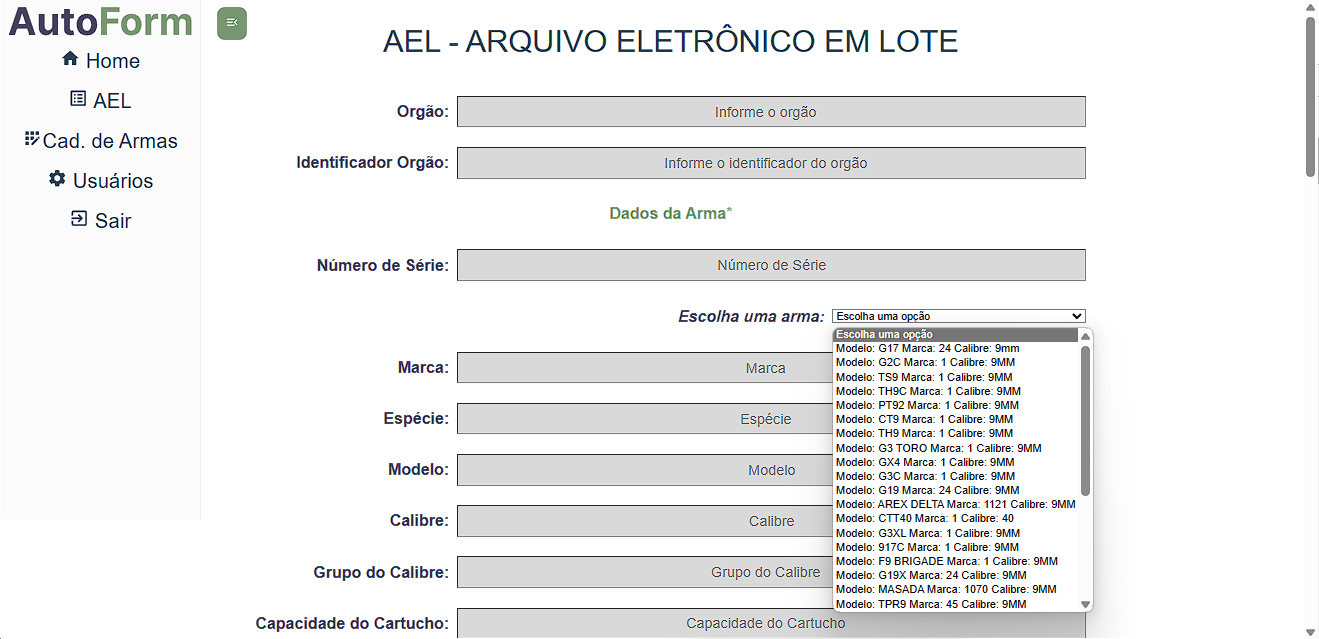
\includegraphics[scale=0.3]{imagens/autoform-ael-selecao.png}
    \end{center}
    \legend{Fonte: Autor}
\end{figure}

\begin{figure}[H]
    \caption{\label{fig:tela-ael2}Autoform - Página criação AEL -2}
    \begin{center}
        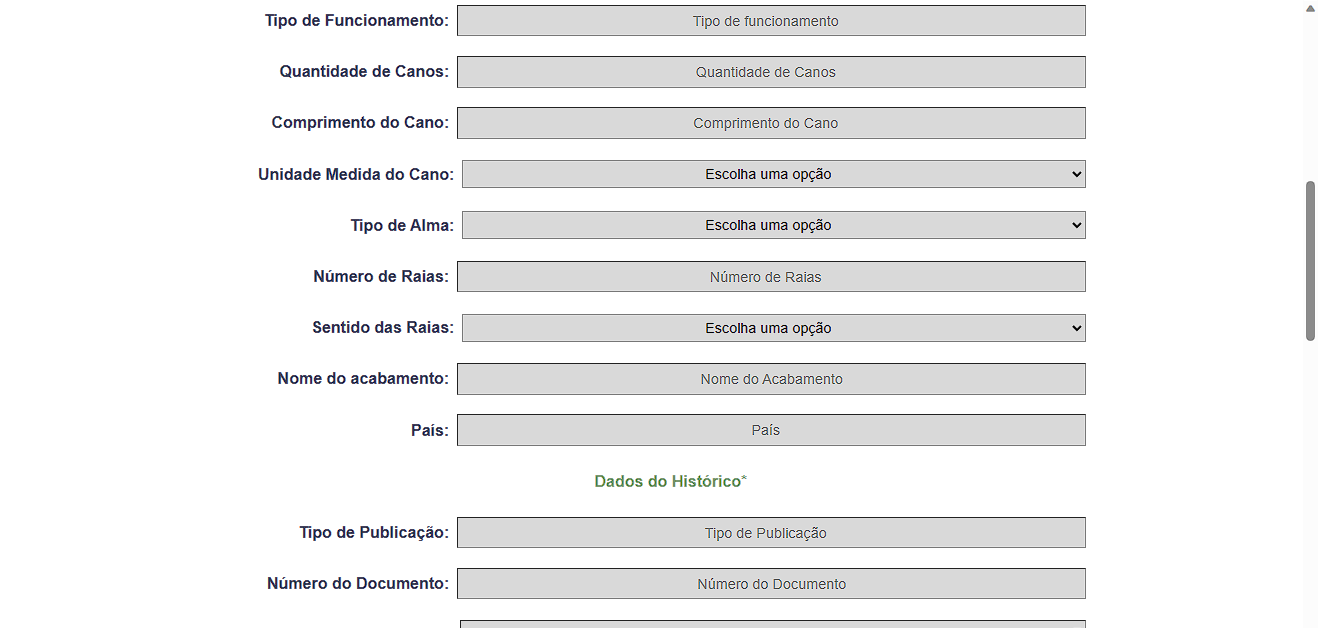
\includegraphics[scale=0.5]{imagens/autoform-ael-gerar2.png}
    \end{center}
    \legend{Fonte: Autor}
\end{figure}
\begin{figure}[H]
    \caption{\label{fig:tela-ael3}Autoform - Página criação AEL-3}
    \begin{center}
        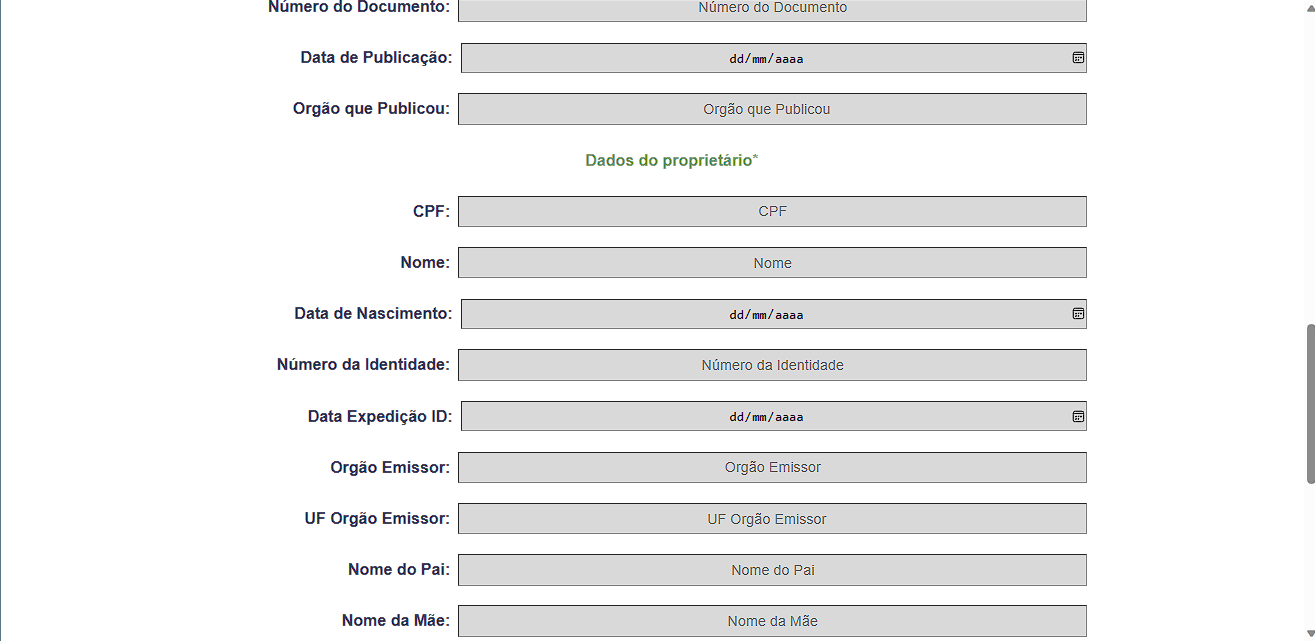
\includegraphics[scale=0.5]{imagens/autoform-ael-gerar3.png}
    \end{center}
    \legend{Fonte: Autor}
\end{figure}

\begin{figure}[H]
    \caption{\label{fig:tela-ael4}Autoform - Página criação AEL-4}
    \begin{center}
        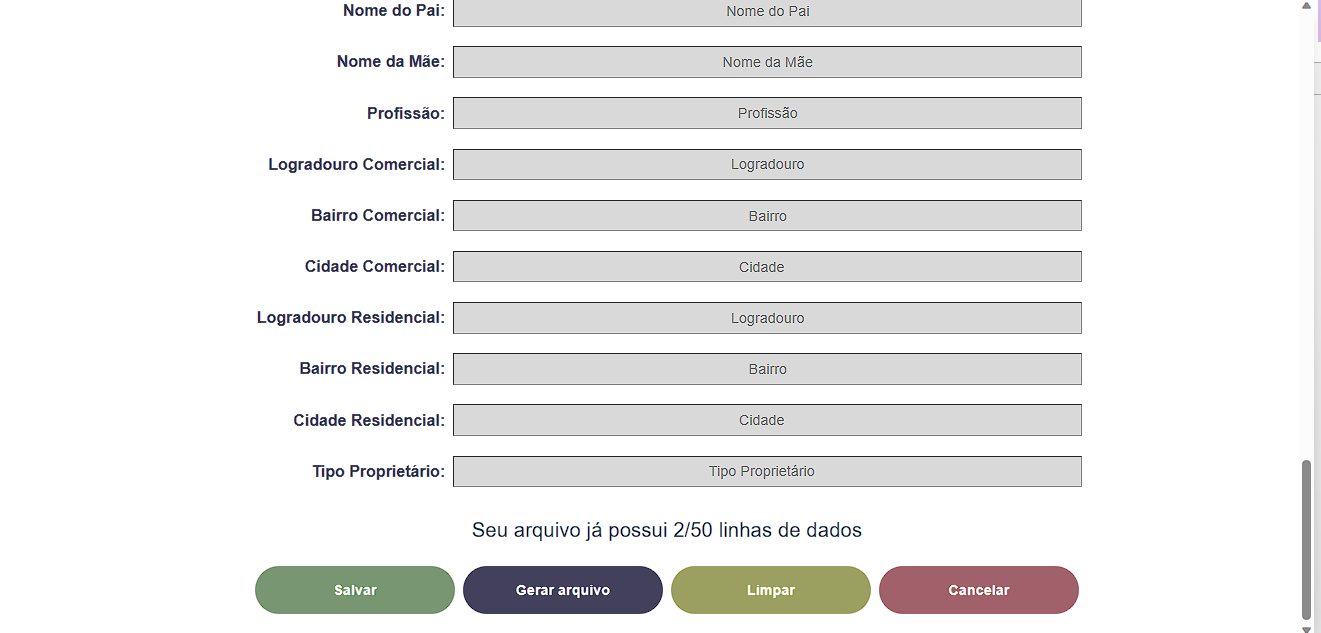
\includegraphics[scale=0.5]{imagens/autoform-ael-gerar4.png}
    \end{center}
    \legend{Fonte: Autor}
\end{figure}

Telas do formulário web para geração do AEL

Os botões da \autoref{fig:tela-ael4} tem as seguintes funcionalidades:
\begin{itemize}
    \item Salvar: Verifica se todos os campos obrigatórios foram preenchidos, e caso estejam preenchidos, salva o registro no \textit{local storage} do navegador.
    \item Gerar Arquivo: Com base nos registros salvos no \textit{local storage}, a aplicação realiza a normalização das informações de acordo com as regras específicas de indexação contidas nos \autoref{sec:anexoA1} e \autoref{sec:anexoA2}.Após pergunta ao usuário o nome do AEL e gera automaticamente o arquivo com base no nome inserido, realizando o download do arquivo AEL para o navegador do usuário que solicitou o recurso. 
    \item Limpar: Este botão exibe uma mensagem perguntando ao usuário se deseja limpar Nº linhas de registros contidos no armazenamento local do navegador.  Após confirmada a ação os registros temporários são apagados. 
    Esta opção foi implementada para garantir que após gerar o arquivo o usuário possa apagar os registros antigos para inserir novos. E também como garantia de segurança, limpando todos os dados do armazenamento temporário para  que não fique nenhuma informação sensível salva no navegador do usuário.
    \item Cancelar: Esse botão tem como intuito apenas direcionar o usuário para a pagina inicial da aplicação a \autoref{fig:tela-home}, saindo da opção de criação de AEL.
\end{itemize}

\subsubsection{Exemplo de AEL gerado}
Exemplo da ação executada após selecionar o botão gerar arquivo, que tem como saída o arquivo AEL formatado.

\begin{figure}[H]
    \caption{\label{fig:tela-ael-gerado}Autoform - AEL gerado}
    \begin{center}
        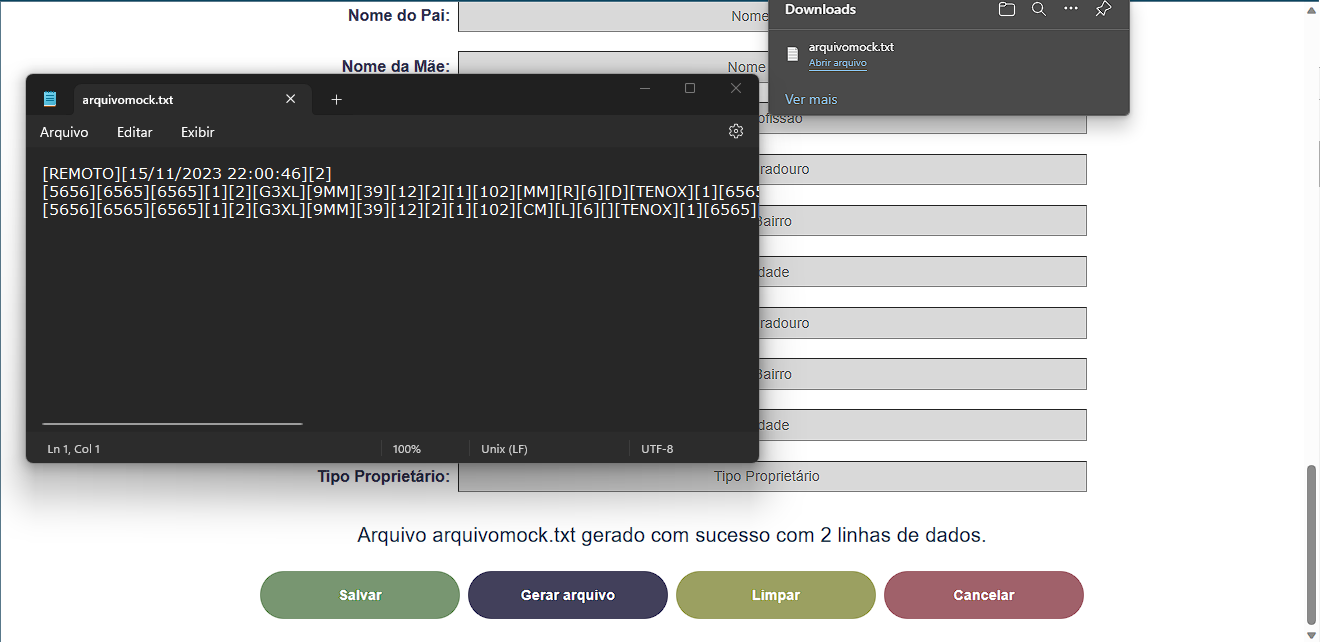
\includegraphics[scale=0.5]{imagens/autoform-ael-gerado.png}
    \end{center}
    \legend{Fonte: Autor}
\end{figure}

\subsubsection{Página de cadastros}
Nesta página é possível visualizar os cadastros de armas que são armazenadas no banco de dados, também é possível realizar uma pesquisa.
\begin{itemize}
    \item Pesquisar: Neste campo é possível realizar uma pesquisa por uma arma específica, e caso seja encontrado o registro, o mesmo será exibido na tabela.
    \item Alterar: Neste botão é possível alterar o registro de arma, e após a edição o registro é atualizado no banco de dados.
    \item Excluir: Neste botão é possível excluir o registro de arma, e após a exclusão o registro é removido do banco de dados.
    \item Cadastrar: Neste botão é possível cadastrar uma nova arma, onde será exibido um modal contendo um formulário para o usuário preencher os dados da arma, e após a confirmação o registro é inserido no banco de dados e uma mensagem de sucesso é exibida ao usuário.
\end{itemize}

\begin{figure}[H]
    \caption{\label{fig:tela-cadastros-armas}Autoform - Cadastros}
    \begin{center}
        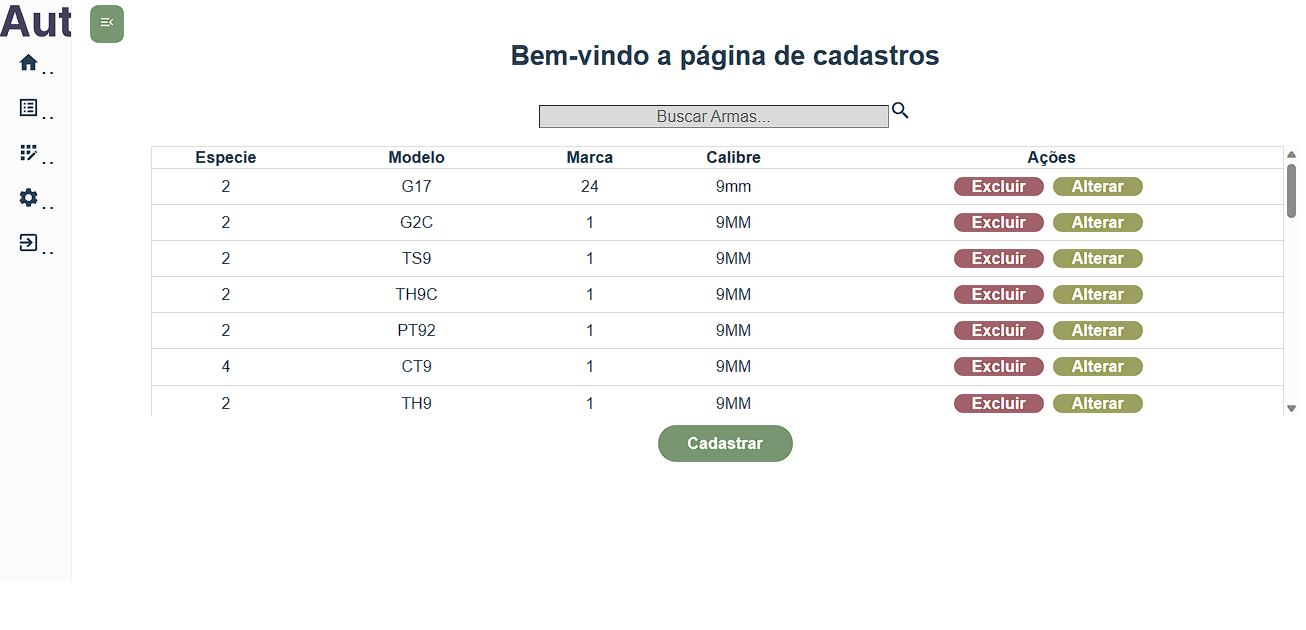
\includegraphics[scale=0.5]{imagens/autoform-cadastros.png}
    \end{center}
    \legend{Fonte: Autor}
\end{figure}

\subsubsection{Página de configurações}
Esta página é acessível somente ao usuário com perfil de administrador.
Nela é exibido o nome, email e status de autorização dos usúarios cadastrados
Sendo possivel realizar o gerenciamento destes através dos seguintes botões:
\begin{itemize}
    \item Pesquisar: Neste campo é possível realizar uma pesquisa por um usuário específico, e caso seja encontrado o registro, o mesmo será exibido na tabela.
    \item Excluir: Neste botão é possível excluir o registro de usuário, e após a confirmação de exclusão o registro é removido do banco de dados.
    \item Alterar senha: Neste botão é possível alterar a senha de usuário, onde será exibido um campo para o administrador informar a nova senha e após a confirmação. O registro é atualizado no banco de dados e uma mensagem de sucesso é exibida ao Usuário
    \item Autorizar: Ao utilizar esse botão é possível alterar o status do usuário para autorizado, liberando o acesso a aplicação. Onde o registro é atualizado no banco de dados e uma mensagem de sucesso é exibida ao usuário.
    \item Bloquear: Ao utilizar esse botão é possível alterar o status do usuário para bloqueado, bloqueando o acesso a aplicação. Onde o registro é atualizado no banco de dados e uma mensagem de sucesso é exibida ao usuário.
\end{itemize}

\begin{figure}[H]
    \caption{\label{fig:tela-configuracoes}Autoform - Configurações}
    \begin{center}
        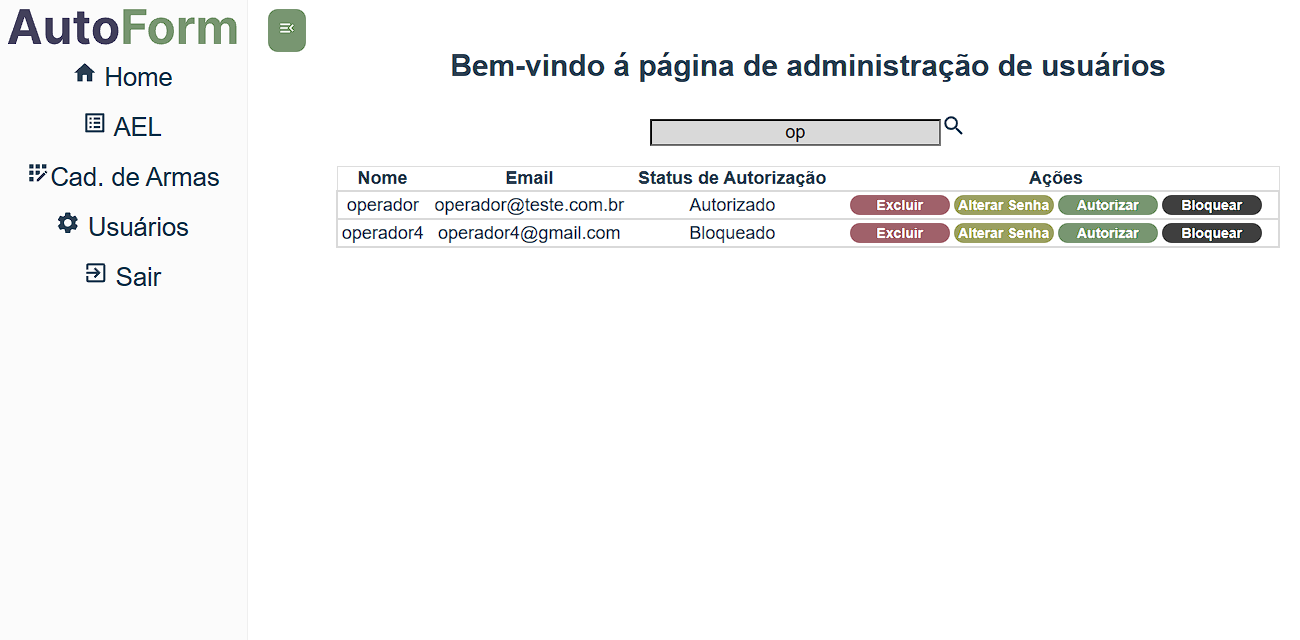
\includegraphics[scale=0.5]{imagens/autoform-configuracoes.png}
    \end{center}
    \legend{Fonte: Autor}
\end{figure}



% Este capítulo possui também exemplos de como inserir código no texto.
% % ---
% \section{Vestibulum ante ipsum primis in faucibus orci luctus et ultrices
% posuere cubilia Curae}
% % ---

% \lipsum[21-22]

% \section{Inserindo código no texto}

% Abaixo são apresentados exemplos de códigos inseridos no texto usando o pacote listings.

% %Inserindo código diretamente no texto
% \begin{lstlisting}[language=c, caption={Exemplo de código C}, upquote=true]
% #include <stdio.h>

% int main(int argc, const char * argv[]) {
% struct pessoa{
% char nome[20];
% char sobreNome[20];
% unsigned short idade;
% char cpf[15];
% }p1;
% //struct pessoa p1;

% printf("Digite o nome: ");
% scanf("%s",p1.nome);
% printf("Digite o sobrenome: ");
% scanf("%s",p1.sobreNome);
% printf("Digite a idade: ");
% scanf("%hu",&p1.idade);
% printf("Digite o CPF: ");
% scanf("%s",p1.cpf);

% printf("\nO nome da pessoa eh: %s", p1.nome);
% printf("\nO sobrenome da pessoa eh: %s", p1.sobreNome);
% printf("\nA idade da pessoa eh: %d", p1.idade);
% printf("\nO CPF da pessoa eh: %s\n", p1.cpf);
% }
% \end{lstlisting}

% \lipsum[1]

% %Ao invés de inserir código diretamente no texto, é recomendável importar um arquivo com o código

% %Importanto arquivo de código
% \lstinputlisting[language=Java,caption={Exemplo de código java}]{codigos/Minhaclasse.java}

% O método abaixo mostra a string mensagem recebida como parametro e retorna um inteiro digitado pelo usuario. Através de tratamento de exceções, o método executará até que o usuário digite um inteiro válido.

% %Para inserir apenas algumas linhas do arquivo
% \lstinputlisting[language=Java, caption={Método LerInteiro}, firstline=39, lastline=54]{codigos/Ferramentas.java}

% \lipsum[2-3]
% ---


% ---
% Conclusão
% ---
\chapter{Conclusão}
O objetivo principal deste trabalho foi desenvolver uma solução que auxiliasse de forma eficaz os operadores da Brigada Militar ao realizar o processo de registro de produtos controlados no SIGMA através do AEL.

Para isso, foram levantadas as informações necessárias, através da elicitação de requisitos , pesquisa exploratória e analise documental para orientar a pesquisa em busca de uma solução eficiente que fosse segura, tivesse disponibilidade de acesso fácil, não armazenasse dados sensíveis, e ainda fosse capaz de minimizar o esforço empregado pelo operador para gerar o arquivo eletrônico.

Portanto o AutoForm, atendeu aos objetivos específicos estabelecidos proporcionando um preenchimento facilitado, através de uma \textit{interface} intuitiva e amigável, disponível de fácil acesso através da \textit{web} e de forma segura, permitindo que diversos usuários realizem acesso simultâneo e ainda, não armazenando dados sensíveis, pois o arquivo é gerado no computador do usuário.

A aplicação possibilita o cadastro de armas para todos os seus utilizadores, bem como o gerenciamento de usuários para o administrador. Viabilizando a supervisão por parte do administrador sobre quais pessoas têm acesso à aplicação.

\subsection{Resultados finais}

Vislumbrando-se uma estimativa de redução no período de preenchimento do formulário ao eleger uma arma previamente cadastrada para autopreencher 15 campos, seguida pela inserção de dados em apenas 24 campos remanescentes, contemplando inclusivamente os opcionais. Alternativamente, pode-se empregar o preenchimento de apenas 17 campos, sendo somente os obrigatórios ,respectivamente, para a composição do arquivo eletrônico, outrora elaborado manualmente. Essa transição se baseia na totalidade de campos, quantificando em 39.


Logo esperasse que através deste trabalho tenha sido possível alavancar ainda mais a excelência operacional da Brigada Militar, contribuindo para a regulamentação dos produtos controlados, e consequentemente para a segurança pública do estado do Rio Grande do Sul.

\section{Trabalhos futuros}
Nesta seção são descritos alguns trabalhos futuros que podem ser realizados para melhorar a aplicação.

Entre estas atualizações fica sugestão da implementação de alguns campos fixos no AEL como: tipo proprietário , orgão, orgão que publicou e profissão do proprietário, que não foram implementados por não serem obrigatórios, mas que podem ser definidos futuramente por se tratar de informações fixas inerentes a instituição, logo irá minimizar ainda mais a quantidade de campos a serem preenchidos.

Na página de configurações seria interessante adicionar uma opção para o administrador poder selecionar algum outro usuário comum e inserir essa permissão especial, para que assim possa ser delegado a outra pessoa a responsabilidade de gerenciar os demais usuários. Também seria interessante a possibilidade de um botão com a opção para cadastrar novos usuários através desta página.

Na página do AEL,fica a sugestão para adicionar um modal que permita visualizar e editar os registros temporários já salvos, para que assim o usuário possa alterar algum dado que tenha sido preenchido incorretamente, ou até mesmo excluir o registro temporário.


% ---


% ---


% ----------------------------------------------------------
% ELEMENTOS PÓS-TEXTUAIS
% ----------------------------------------------------------
\postextual
% ----------------------------------------------------------

% ----------------------------------------------------------
% Referências bibliográficas (Obrigatório)
% ----------------------------------------------------------
\bibliography{elementos-pos-textuais/referencias}


% ----------------------------------------------------------
% Glossário (Opcional)
% ----------------------------------------------------------
%
% Consulte o manual da classe abntex2 para orientações sobre o glossário.
%
%\glossary


% ----------------------------------------------------------
% Apêndices (Opcional)
% ----------------------------------------------------------
% ---
% Inicia os apêndices
% ---
% \begin{apendicesenv}

% % ----------------------------------------------------------
\chapter{Quisque libero justo}
% ----------------------------------------------------------

\lipsum[50]
% % ----------------------------------------------------------
\chapter{Nullam elementum urna vel imperdiet sodales elit ipsum pharetra ligula
ac pretium ante justo a nulla curabitur tristique arcu eu metus}
% ----------------------------------------------------------
\lipsum[55-57]

% \end{apendicesenv}
% ---


% ----------------------------------------------------------
% Anexos (Opcional)
% ----------------------------------------------------------
% ---
% Inicia os anexos
% ---
\begin{anexosenv}

\chapter{\textit{Portaria 136 - Anexo D.1}}
\label{sec:anexoA1}

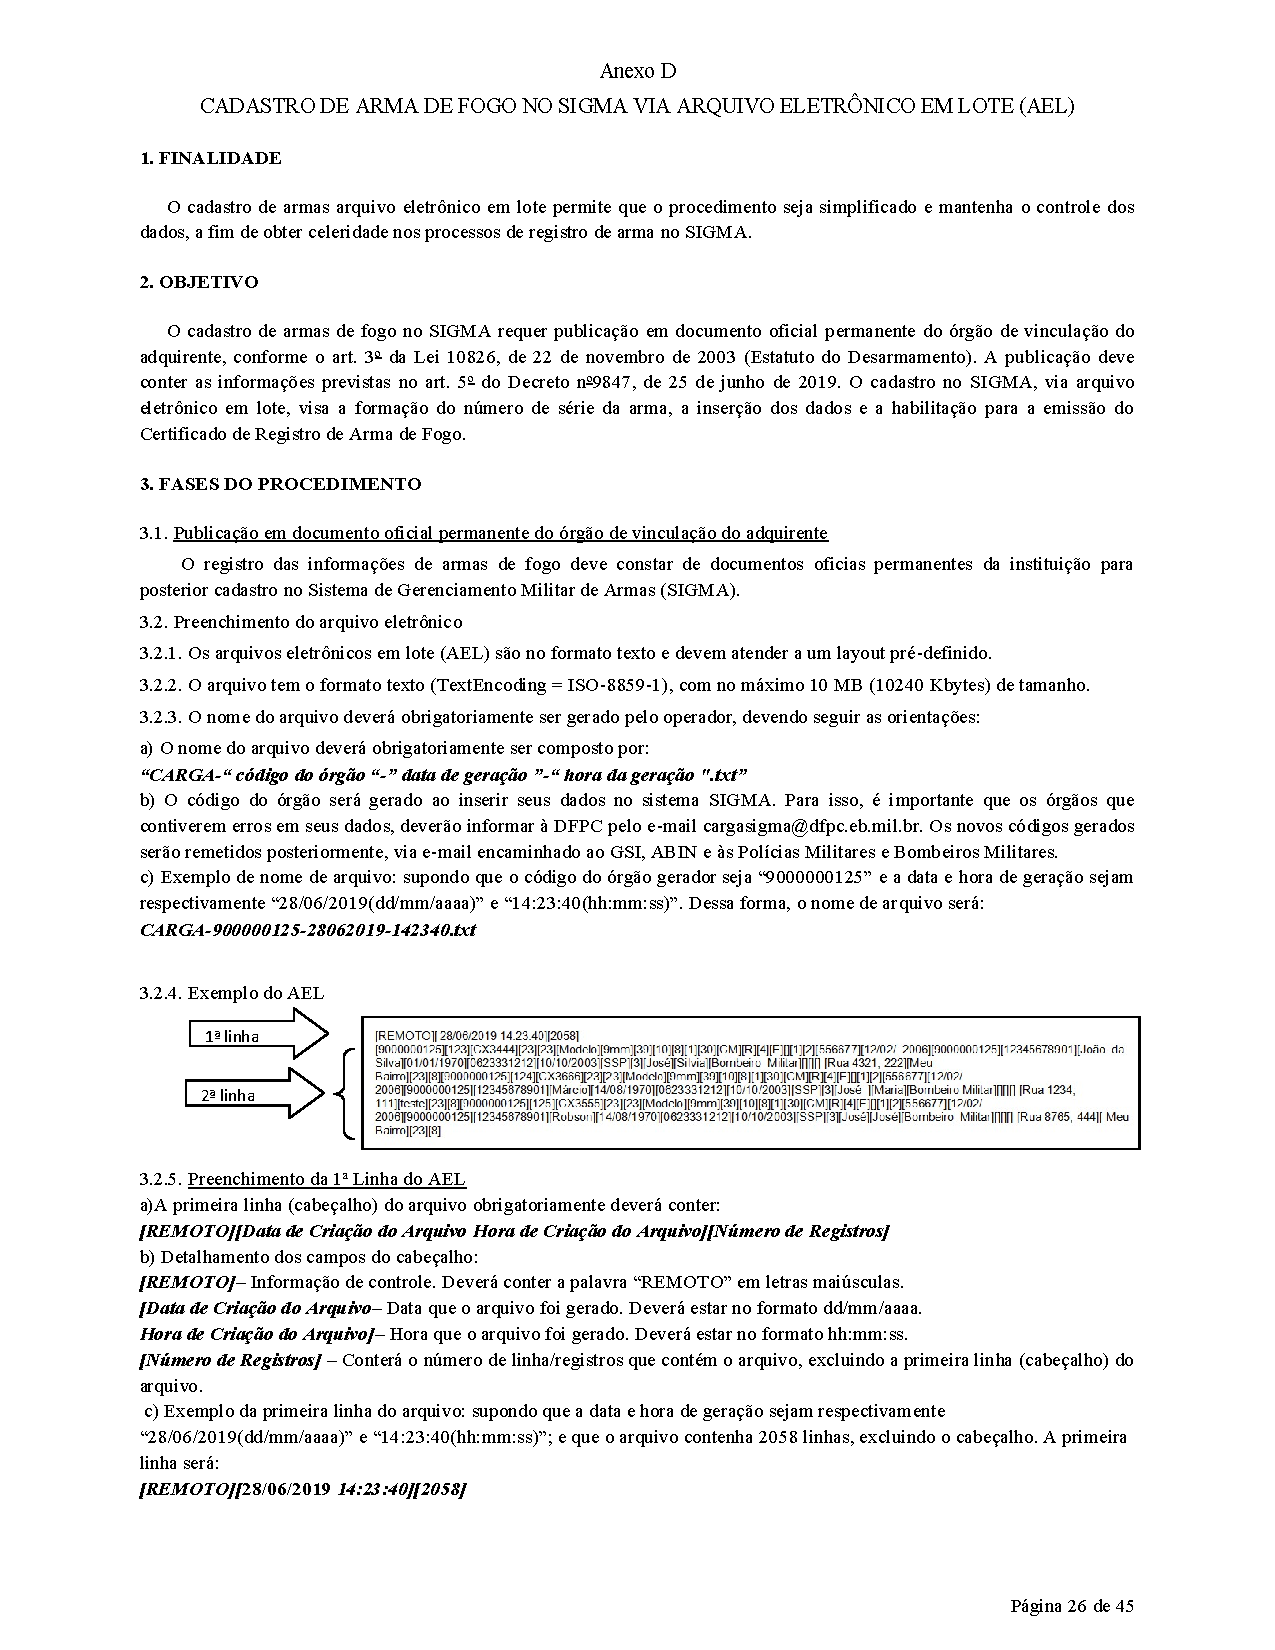
\includegraphics[scale=0.8]{imagens/AnexoA1-AnexoD-portaria-136}




% ---
\chapter{Portaria 136 - Anexo D - Página 27}
% ---
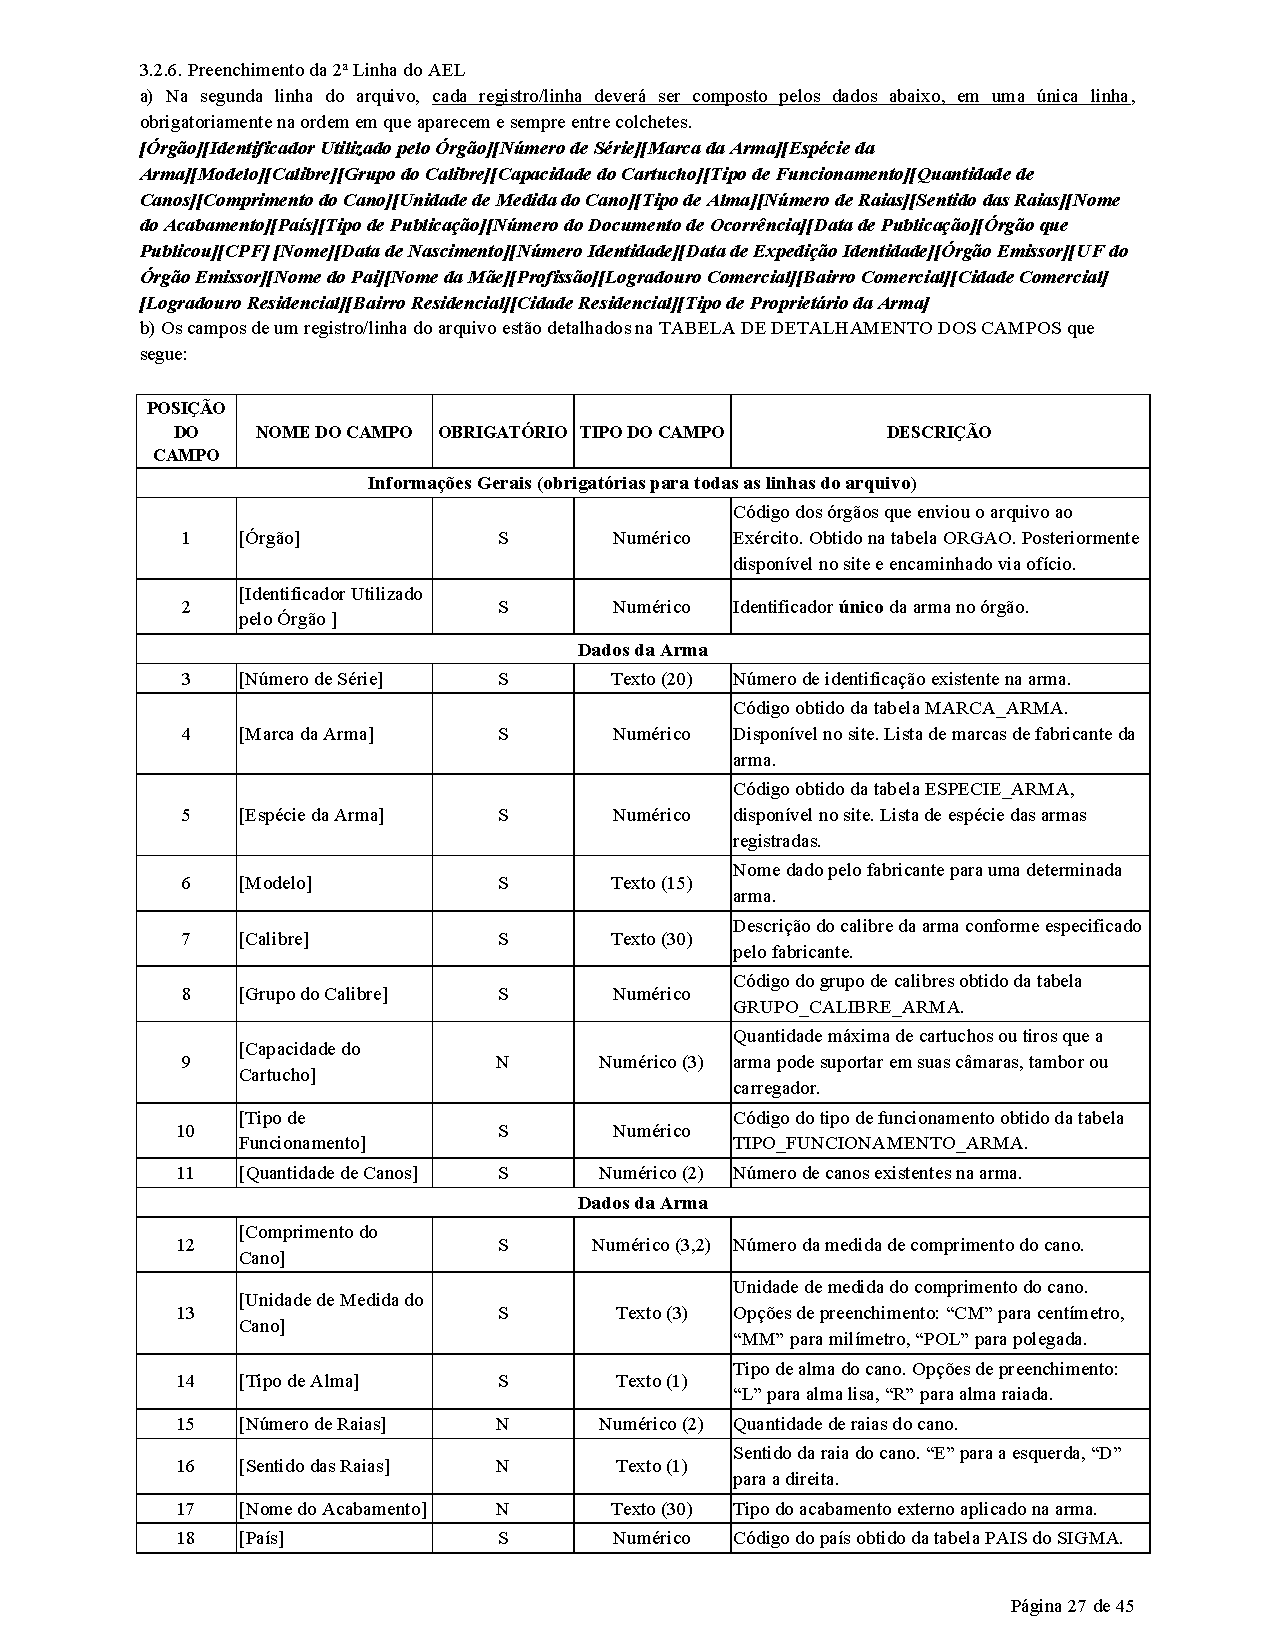
\includegraphics[scale=0.7]{imagens/AnexoA2-AnexoD-portaria-136}


% ---
\chapter{\textit{Portaria 136 - Anexo D.3}}
\label{sec:anexoA3}
% ---
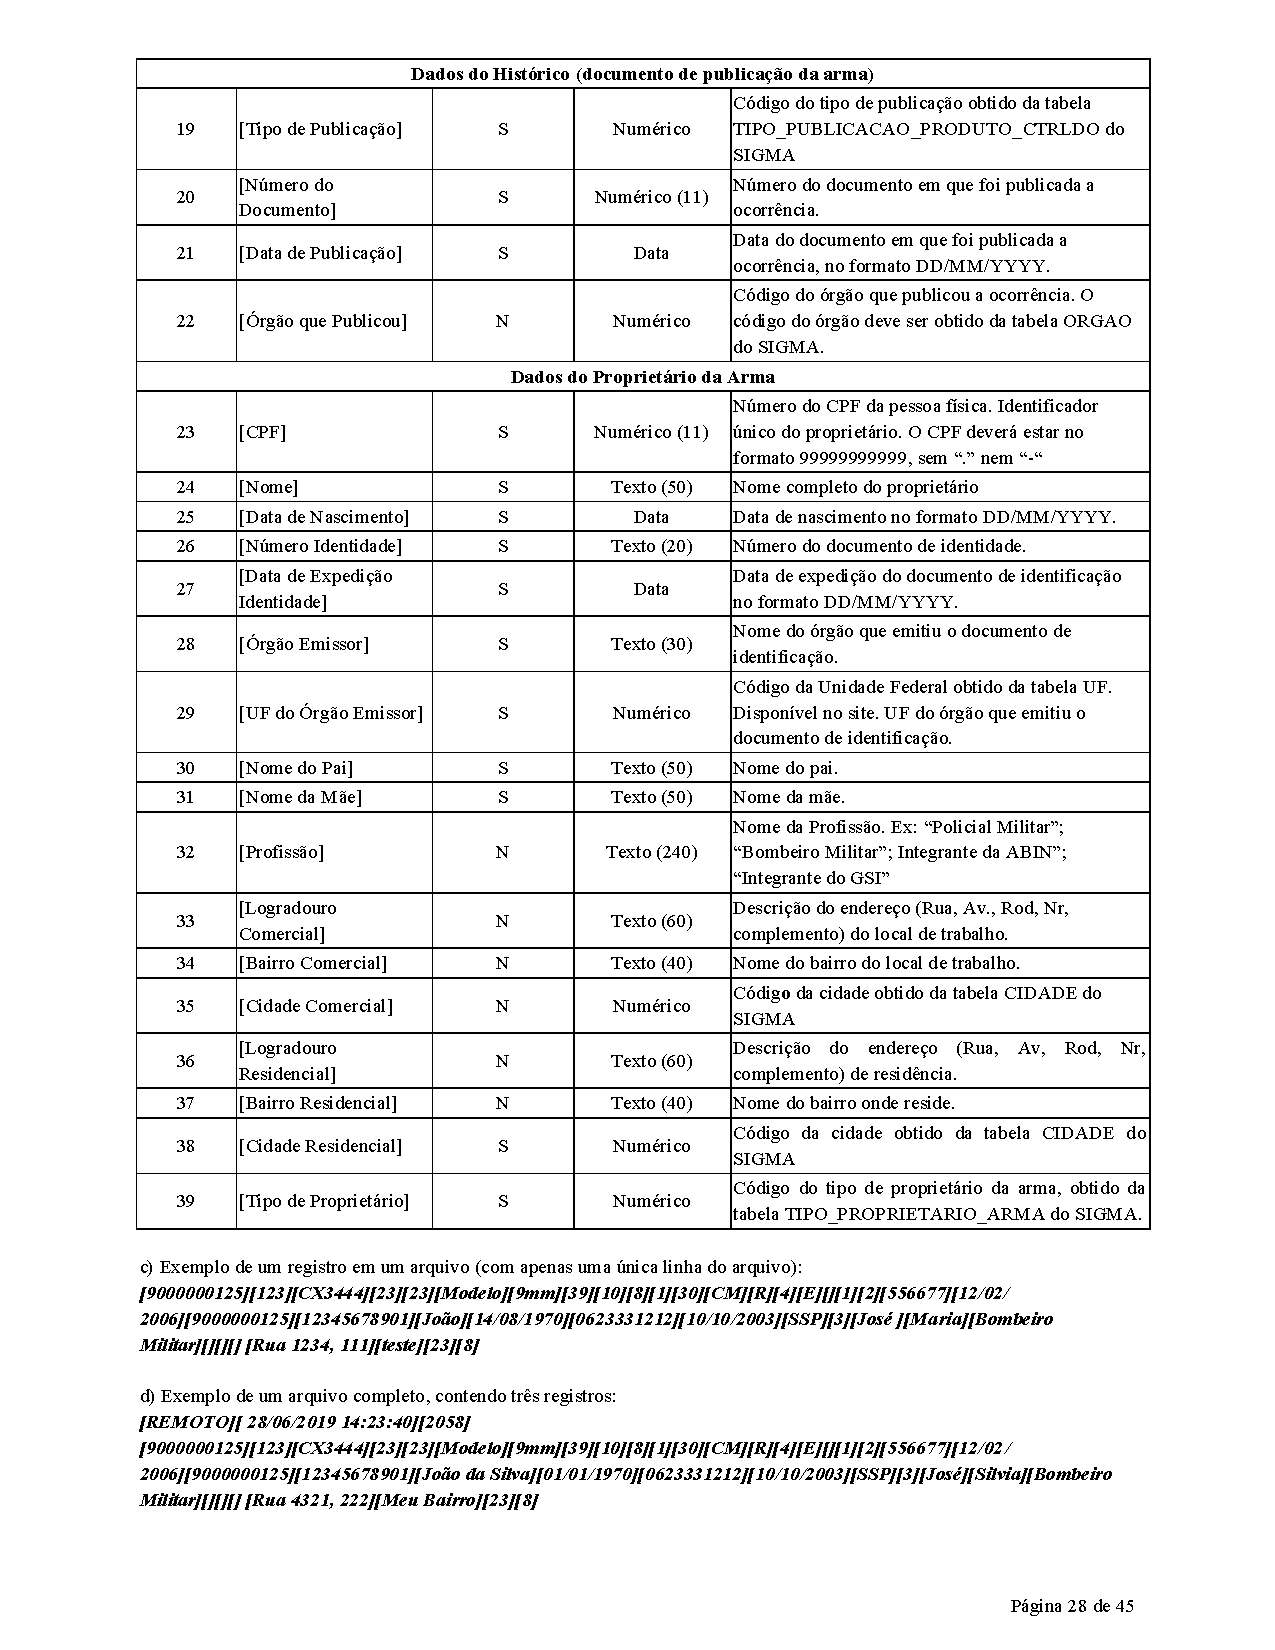
\includegraphics[scale=0.8]{imagens/AnexoA3-AnexoD-portaria-136}


% ---
\chapter{\textit{Portaria 136 - Anexo D - Página 29}}
% ---
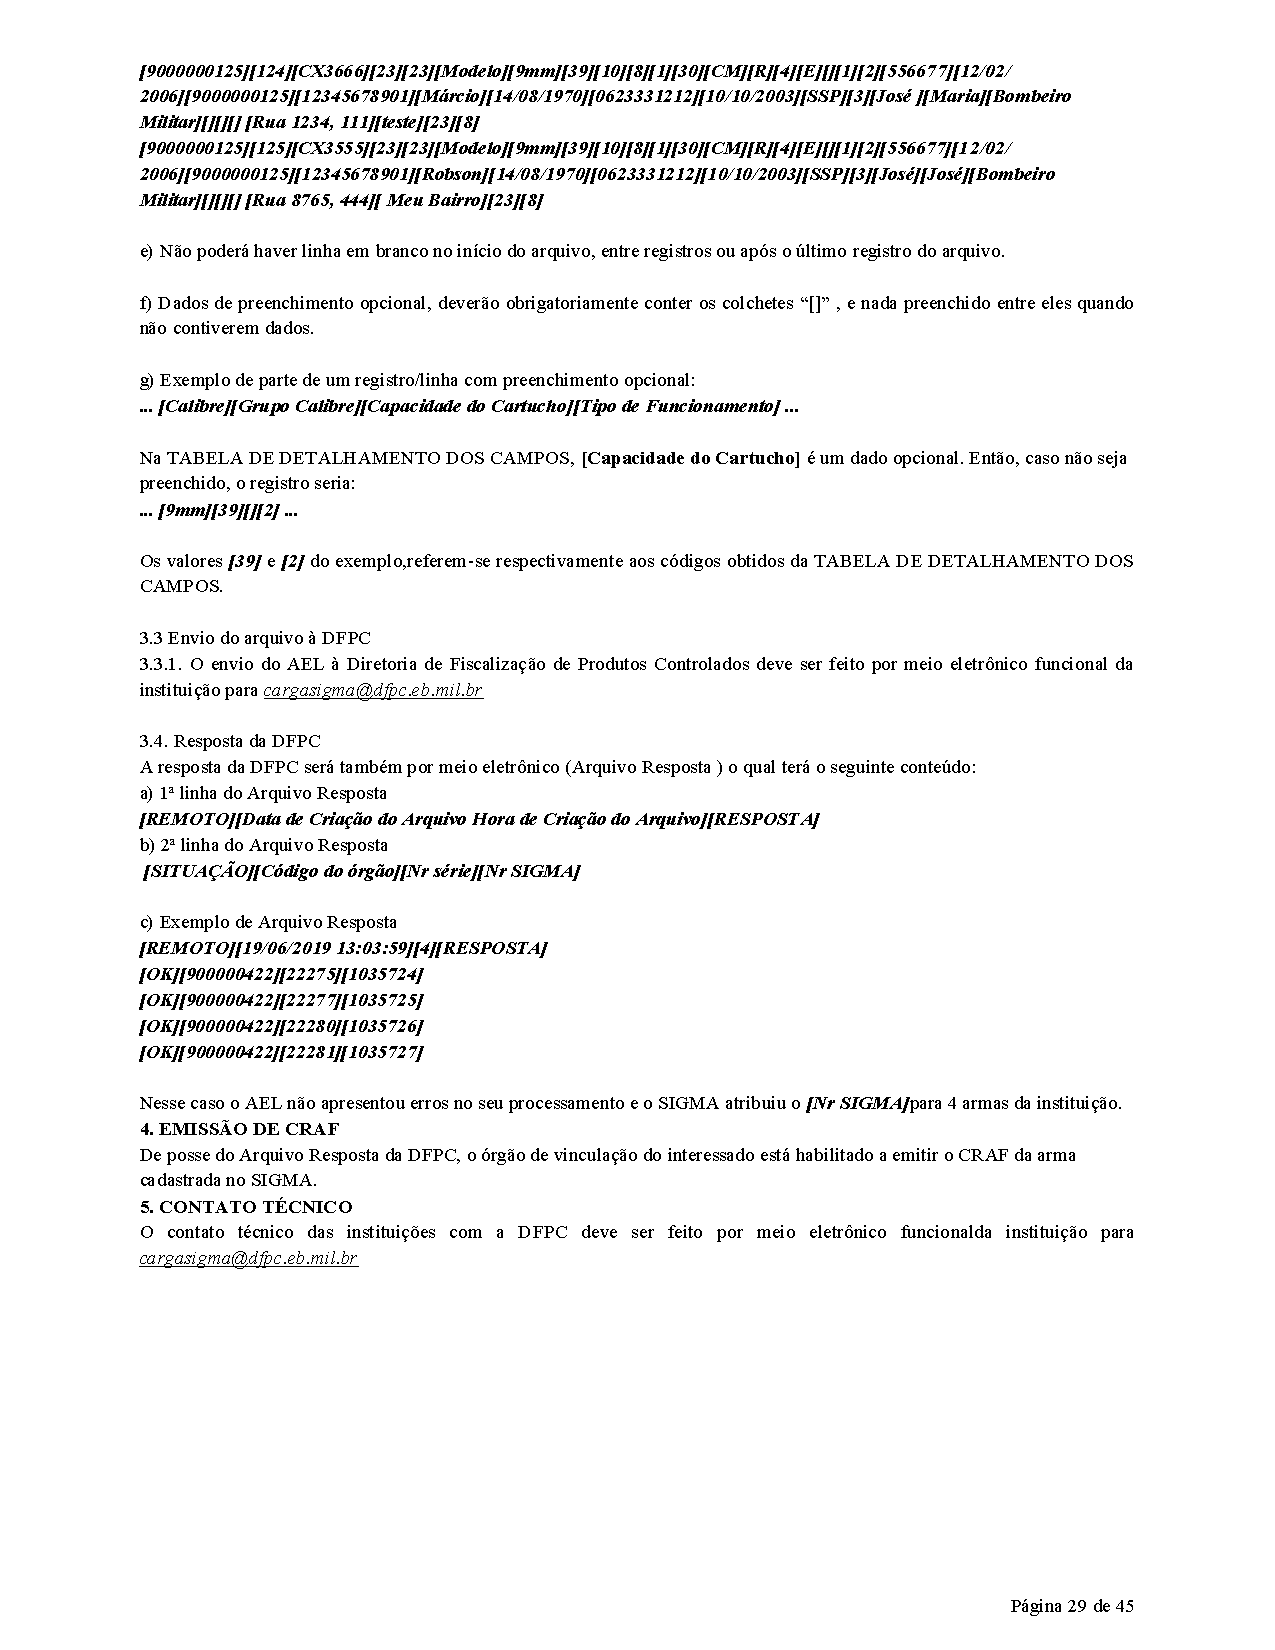
\includegraphics[scale=0.8]{imagens/AnexoA4-AnexoD-portaria-136}


\end{anexosenv}


%---------------------------------------------------------------------
% INDICE REMISSIVO (Opcional)
%---------------------------------------------------------------------
%\phantompart
%\printindex
%---------------------------------------------------------------------

\end{document}
